\documentclass[]{article}
\usepackage{geometry,tikz,lipsum,amsmath,amssymb,soul,xcolor,cancel}
\tikzset{every picture/.style={line width=0.75pt}} %set default line width to 0.75pt        
\numberwithin{equation}{section}

\NewDocumentCommand{\caja}{ m O{gray!40} O{gray!10} m }{
	\begin{figure}[h]
		\centering
		\begin{tikzpicture}
			\node[anchor=text, text width=\columnwidth-1.2cm, draw, rounded corners, line width=1pt, fill=#3, inner sep=5mm] (big) {\\#4};
			\node[draw, rounded corners, line width=.5pt, fill=#2, anchor=west, xshift=5mm] (small) at (big.north west) {#1};
		\end{tikzpicture}
	\end{figure}
}

\newcommand{\deriv}[3]{\left(\frac{\partial #1}{\partial #2} \right)_{#3}}

\newcommand{\dderiv}[3]{\left(\dfrac{\partial #1}{\partial #2} \right)_{#3}}

%opening
\title{Física Estadística Avanzada}
\author{Simon Fonseca}

\begin{document}

\maketitle

\section{Termodinámica}
\subsection{Ley cero}
\caja{Equilibrio térmico}{Dos sistemas en contacto están en equilibrio térmico cuando no hay flujo neto de energía térmica.}

Si tenemos 3 sistemas $A$, $B$ y $C$ en contacto secuencial y se cumple que:
\begin{enumerate}
	\item $A$ y $B$ están en equilibrio térmico.
	\item $B$ y $C$ están en equilibrio térmico.
	\item[$\Rightarrow$] Entonces, $A$ y $C$ están en equilibrio térmico.
\end{enumerate}

\begin{figure}[h]
	\centering      
	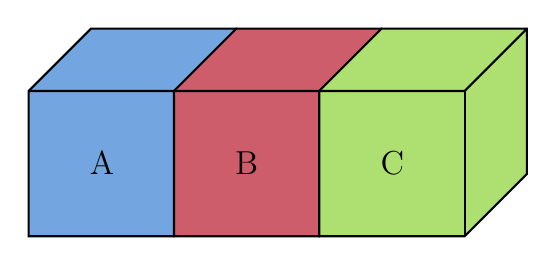
\begin{tikzpicture}[x=0.75pt,y=0.75pt,yscale=-1,xscale=1]
		%uncomment if require: \path (0,300); %set diagram left start at 0, and has height of 300
		
		%Shape: Cube [id:dp9619949875210992] 
		\draw  [fill={rgb, 255:red, 115; green, 165; blue, 224 }  ,fill opacity=1 ] (40,60) -- (70,30) -- (140,30) -- (140,100) -- (110,130) -- (40,130) -- cycle ; \draw   (140,30) -- (110,60) -- (40,60) ; \draw   (110,60) -- (110,130) ;
		%Shape: Cube [id:dp7736464687520493] 
		\draw  [fill={rgb, 255:red, 206; green, 93; blue, 108 }  ,fill opacity=1 ] (110,60) -- (140,30) -- (210,30) -- (210,100) -- (180,130) -- (110,130) -- cycle ; \draw   (210,30) -- (180,60) -- (110,60) ; \draw   (180,60) -- (180,130) ;
		%Shape: Cube [id:dp6377409033689178] 
		\draw  [fill={rgb, 255:red, 173; green, 224; blue, 113 }  ,fill opacity=1 ] (180,60) -- (210,30) -- (280,30) -- (280,100) -- (250,130) -- (180,130) -- cycle ; \draw   (280,30) -- (250,60) -- (180,60) ; \draw   (250,60) -- (250,130) ;
		
		% Text Node
		\draw (68,88) node [anchor=north west][inner sep=0.75pt]   [align=left] {\large{A}};
		% Text Node
		\draw (138,88) node [anchor=north west][inner sep=0.75pt]   [align=left] {\large{B}};
		% Text Node
		\draw (208,88) node [anchor=north west][inner sep=0.75pt]   [align=left] {\large{C}};
		
		
	\end{tikzpicture}
\end{figure}

\caja{Temperatura ($T$)}{Es una propiedad macroscópica y medible del sistema que determina el sentido del flujo de energía. Es igual entre sistemas en equilibrio térmico.}

\caja{Calor ($Q$)}{Es una transferencia de energía que ocurre entre dos sistemas que no están en equilibrio térmico. La energía se puede transferir de dos formas: trabajo ($W$) y calor ($Q$). Mientras que el trabajo es ejercido a través de fuerzas externas, como mecánicas o eléctricas, el calor engloba la energía transferida por otros medios.}

\subsection{Primera ley}
\subsubsection{Diferenciales inexactos ($\delta$)}
Matemáticamente, un diferencial es un objeto llamado 1-forma diferencial $\omega$, el cual puede expresarse, en el caso que dependa de dos variables $x, y$ como:
\begin{equation}
	\omega = M(x,y)dx + N(x,y)dy
\end{equation}

Le diremos diferencial \textit{exacto} ($d$) al tipo "común" de diferencial de Cálculo 1. Es una subtipo de 1-forma que cumple con ser la derivada exterior de alguna función escalar continua $f(x,y)$. Si vemos el objeto $df$ sabremos que siempre podremos escribir algo en la forma:
\begin{equation}
	\omega = df = \frac{\partial f}{\partial x}(x,y)dx  + \frac{\partial f}{\partial y}(x,y)dy,
	\label{eqn:def_dif_exacto}
\end{equation}
lo cual, en este caso, implica la existencia de una ecuación "maestra" que existe como una superficie en el espacio 3-D.

Por el contrario, un diferencial \textit{inexacto} ($\delta$) será el caso por defecto de una 1-forma, donde las funciones $M(x,y), N(x,y)$ no representan derivadas parciales de ninguna función, ya que no existe una superficie $f(x,y)$ que la defina.
\begin{equation}
	\omega = \delta W = M(x,y)dx + N(x,y)dy
\end{equation}

Como consecuencia de esto, y ya que el orden de diferenciación no importa para ecuaciones continuas, tendremos que:
\begin{align}
	\frac{\partial^2 f}{\partial x\partial y}(x,y) &= \frac{\partial^2 f}{\partial y\partial x}(x,y)\label{eqn:orden_dif}\\
	\Rightarrow \frac{\partial M}{\partial y}(x,y) &= \frac{\partial N}{\partial x}(x,y)\label{eqn:orden_dif2}
\end{align}
si y solo si $\omega$ es un diferencial \textbf{exacto}.

\begin{figure}[h!]
	\centering
	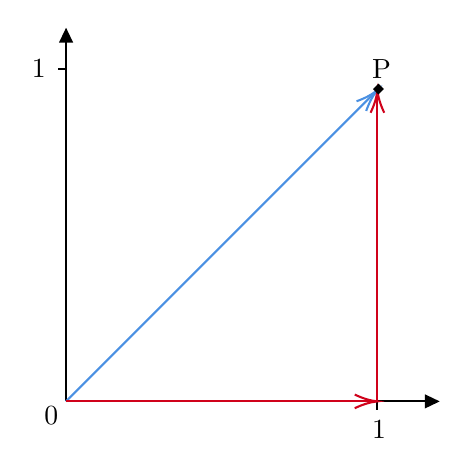
\begin{tikzpicture}[x=0.75pt,y=0.75pt,yscale=-1,xscale=1]
		%uncomment if require: \path (0,300); %set diagram left start at 0, and has height of 300
		
		%Straight Lines [id:da11893720987770351] 
		\draw    (30,210) -- (31.31,210) -- (207,210) ;
		\draw [shift={(210,210)}, rotate = 180] [fill={rgb, 255:red, 0; green, 0; blue, 0 }  ][line width=0.08]  [draw opacity=0] (7.14,-3.43) -- (0,0) -- (7.14,3.43) -- cycle    ;
		%Straight Lines [id:da3885266277462476] 
		\draw    (30,210) -- (30,33) ;
		\draw [shift={(30,30)}, rotate = 90] [fill={rgb, 255:red, 0; green, 0; blue, 0 }  ][line width=0.08]  [draw opacity=0] (7.14,-3.43) -- (0,0) -- (7.14,3.43) -- cycle    ;
		%Straight Lines [id:da6222388127714078] 
		\draw    (180,210) -- (180,214) ;
		%Straight Lines [id:da5056121738009597] 
		\draw    (30,50) -- (26,50) ;
		%Straight Lines [id:da9317710158065218] 
		\draw [color={rgb, 255:red, 74; green, 144; blue, 226 }  ,draw opacity=1 ]   (30,210) -- (178.59,61.41) ;
		\draw [shift={(180,60)}, rotate = 135] [color={rgb, 255:red, 74; green, 144; blue, 226 }  ,draw opacity=1 ][line width=0.75]    (10.93,-3.29) .. controls (6.95,-1.4) and (3.31,-0.3) .. (0,0) .. controls (3.31,0.3) and (6.95,1.4) .. (10.93,3.29)   ;
		%Straight Lines [id:da16708685670753765] 
		\draw [color={rgb, 255:red, 208; green, 2; blue, 27 }  ,draw opacity=1 ]   (30,210) -- (178,210) ;
		\draw [shift={(180,210)}, rotate = 180] [color={rgb, 255:red, 208; green, 2; blue, 27 }  ,draw opacity=1 ][line width=0.75]    (10.93,-3.29) .. controls (6.95,-1.4) and (3.31,-0.3) .. (0,0) .. controls (3.31,0.3) and (6.95,1.4) .. (10.93,3.29)   ;
		%Straight Lines [id:da0884937632478392] 
		\draw [color={rgb, 255:red, 208; green, 2; blue, 27 }  ,draw opacity=1 ]   (180,210) -- (180,62) ;
		\draw [shift={(180,60)}, rotate = 90] [color={rgb, 255:red, 208; green, 2; blue, 27 }  ,draw opacity=1 ][line width=0.75]    (10.93,-3.29) .. controls (6.95,-1.4) and (3.31,-0.3) .. (0,0) .. controls (3.31,0.3) and (6.95,1.4) .. (10.93,3.29)   ;
		%Flowchart: Connector [id:dp49107358933661316] 
		\draw  [color={rgb, 255:red, 0; green, 0; blue, 0 }  ,draw opacity=1 ][fill={rgb, 255:red, 0; green, 0; blue, 0 }  ,fill opacity=1 ][line width=2.25]  (180,59.5) .. controls (180,59.22) and (180.22,59) .. (180.5,59) .. controls (180.78,59) and (181,59.22) .. (181,59.5) .. controls (181,59.78) and (180.78,60) .. (180.5,60) .. controls (180.22,60) and (180,59.78) .. (180,59.5) -- cycle ;
		
		% Text Node
		\draw (12,44) node [anchor=north west][inner sep=0.75pt]   [align=left] {1};
		% Text Node
		\draw (176,218) node [anchor=north west][inner sep=0.75pt]   [align=left] {1};
		% Text Node
		\draw (18,211) node [anchor=north west][inner sep=0.75pt]   [align=left] {0};	
		% Text Node
		\draw (176,44) node [anchor=north west][inner sep=0.75pt]   [align=left] {P};	
	\end{tikzpicture}
	\label{fig:ejemplo_path}
\end{figure}

Además, las cantidades inexactas serán independientes del camino de integración. Por ejemplo, si tenemos:
\begin{equation*}
	\delta F = xy dx + x^2 dy
\end{equation*}
e integramos de 0 al punto $P$ por dos caminos distintos, como se ve en la figura \ref{fig:ejemplo_path}, obtendremos:
\begin{align*}
	&\textcolor{blue}{\int_{0}^{P}F_x dx + F_y dy,\ \ \ r=x=y,\ \ \ dr=dx=dy,\ \ \ t:0 \rightarrow 1}\\
	\textcolor{blue}{=}&\textcolor{blue}{\int_{0}^{1}(r\cdot r+r^2)dr = \frac{2}{3}}\\
	&\textcolor{red}{\int_{0}^{1}F_x(x,0) dx + \int_{0}^{1} F_y(1,y) dy}\\
	\textcolor{red}{=}&\textcolor{red}{\int_{0}^{1}(x\cdot 0)dx + \int_{0}^{1}(1^2)dy = 0+1 = 1}
\end{align*}
La integral dependerá del camino tomado.

En nuestro caso, los diferenciales inexactos representarán cantidades "en tránsito", como el trabajo o el calor, para las cuales no se pueden definir cantidades absolutas pero sí flujos.

\subsubsection{Primera Ley}
\caja{Energía interna ($E$)}{En un sistema termodinámico, es la suma de toda la energía cinética y potencial poseída por sus partículas constituyentes.}

La energía interna solo puede cambiar a través de trabajo o calor. Es decir,
\begin{equation}
	\Delta E = Q+W
\end{equation}
o, para un proceso infinitesimal
\begin{equation}
	dE = \delta Q + \delta W
\end{equation}

Para dos sistemas aislados, se comprueba experimentalmente que el calor transferido se conserva, es decir, el calor que sale del sistema a mayor temperatura es igual al que entra al sistema de menor temperatura.

Ya que la temperatura afecta otras propiedades de un cuerpo, podemos medirla indirectamente sabiendo la relación con alguna otra propiedad. En el caso del termómetro de alcohol, se puede utilizar su relación con dilatación lineal y volumétrica:
\begin{equation}
	\begin{matrix}
		L\rightarrow L_0+\Delta L & & V\rightarrow V_0+\Delta V\\
		\Delta L = L_0\alpha\Delta T & & \Delta V \approx V_0\beta\Delta T 
	\end{matrix}
\end{equation}
donde $\alpha$ y $\beta$ dependen de cada sustancia.

\subsubsection{Capacidad calórica}
\caja{Capacidad calórica y calor específico}{Un cuerpo hecho de una sustancia cualquiera se dirá que tiene una capacidad calórica $C$ si necesita de $C$ unidades de calor para aumentar su temperatura en 1°C. Por el otro lado, una sustancia se dirá que tiene calor específico $c$ necesita de $c$ unidades de calor para aumentar la temperatura de \textit{una unidad de volumen} en un 1°C.}

El calor específico del agua líquida está definido en
\begin{equation*}
	c_{Agua} = 1 [\text{cal}/(\text{g}\cdot \text{°C})]
\end{equation*}
donde 1 caloría (cal) = 4.18 Joules (J).

Si seguimos agregando calor a un cuerpo mientras mantenemos la presión constante, llegaremos a una temperatura específica de \textbf{cambio de fase}. A partir de este punto, el calor absorbido no produce cambios de temperatura, mas es usado para cambiar de fase (el enlace entre las moléculas del cuerpo). Tendremos que:
\begin{equation}
	Q = M\cdot L_f,
\end{equation}
donde $M$ es la masa del cuerpo y $L_f$ es el \textbf{calor latente} de la fase de sustancia.

\subsubsection{Procesos termodinámicos}
\caja{Presión de un gas}{Se define la presión de un gas como la fuerza por unidad de área ejercida por las partículas constituyentes sobre las paredes del recipiente.}

Si tenemos un gas que se expande a pasos infinitesimales (para poder definir una ecuación de equilibrio en cada instante) tendremos que el trabajo ejercido por el gas será:
\begin{equation}
	W_{\text{by gas}} = \int_{V_{\text{in}}}^{V_{\text{out}}}pdV
\end{equation}
donde $p$ varía con $V$ dependiendo del proceso\footnote{Prueba: de mecánica sabemos que $\delta W = F\cdot dr$, y que $F=P\cdot A$. Luego: $\delta W = (P\cdot A)\cdot dr$, pero área por desplazamiento es volumen, por lo que: $\delta W = P\cdot dV$.}.

En el caso de un gas ideal tendremos la ecuación de estado:
\begin{equation}
	pV=NkT,
	\label{eqn:gases_ideales}
\end{equation}
donde $N$ es la cantidad de moléculas y $k$ es la constante de Boltzmann ($1.38066 \cdot 10^{-23} $[J/K]). Utilizando esta ecuación podremos calcular el trabajo ejercido por el gas, siempre y cuando conozcamos la trayectoria que toma en el espacio de variables.

Podemos definir varios casos especiales definidos por la forma de la curva $T$ a medida que cambia $V$, por ejemplo:
\begin{itemize}
	\item Isotérmico ($T=$ cte.)
	\item Isobárico ($p=$ cte.)
	\item Isocórico ($V=$ cte.)
	\item Adiabático ($Q=0$)
\end{itemize}

\subsubsection{Reversibilidad}
\caja{Proceso cuasiestático}{Si realizamos un proceso termodinámico a pasos infinitesimales tendremos que en cada instante de tiempo podremos definir a todas las variables de estado, y estas cumplirán con las mismas relaciones del sistema en equilibrio. Un proceso cuasiestático es, entonces, reversible e idealizado.}

En procesos irreversibles los estados intermedios no estarán siempre bien definidos por las variables de estado, es decir, la curva que relaciona a las variables no es continua.

Si comprimimos un gas aislado adiabáticamente, $T$ aumenta. Si luego lo dejamos expandirse adiabáticamente, $T$ disminuye. Si realizamos este proceso lentamente el proceso será reversible y al final del ciclo llegaremos a la misma $T$ inicial. En cambio, si comprimimos rápidamente, la $T$ final será mayor y el trabajo ejercido sobre el gas será mayor que en el caso reversible.

\begin{figure}[h]
	\centering
	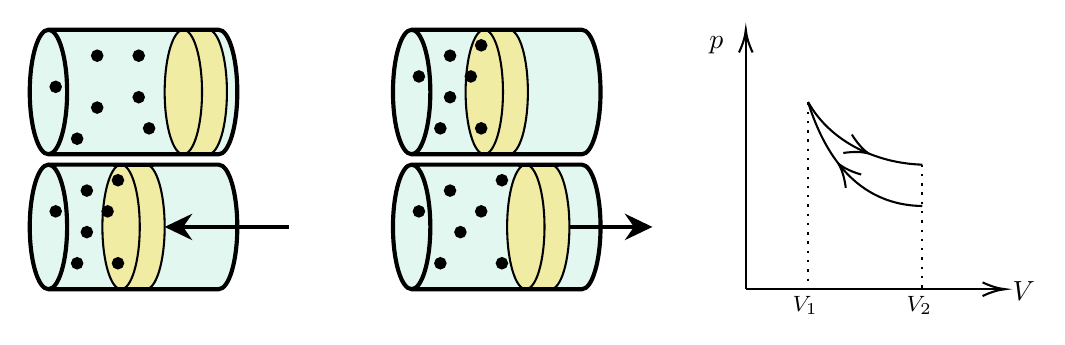
\begin{tikzpicture}[x=0.75pt,y=0.75pt,yscale=-1,xscale=1]		
		%Shape: Can [id:dp015738245941037565] 
		\draw  [fill={rgb, 255:red, 226; green, 247; blue, 239 }  ,fill opacity=1 ][line width=1.5]  (29,20) -- (111,20) .. controls (115.97,20) and (120,33.43) .. (120,50) .. controls (120,66.57) and (115.97,80) .. (111,80) -- (29,80) .. controls (24.03,80) and (20,66.57) .. (20,50) .. controls (20,33.43) and (24.03,20) .. (29,20) .. controls (33.97,20) and (38,33.43) .. (38,50) .. controls (38,66.57) and (33.97,80) .. (29,80) ;
		%Shape: Circle [id:dp047490670873204355] 
		\draw  [fill={rgb, 255:red, 0; green, 0; blue, 0 }  ,fill opacity=1 ] (50,32.5) .. controls (50,31.12) and (51.12,30) .. (52.5,30) .. controls (53.88,30) and (55,31.12) .. (55,32.5) .. controls (55,33.88) and (53.88,35) .. (52.5,35) .. controls (51.12,35) and (50,33.88) .. (50,32.5) -- cycle ;
		%Shape: Circle [id:dp5141101621791769] 
		\draw  [fill={rgb, 255:red, 0; green, 0; blue, 0 }  ,fill opacity=1 ] (70,52.5) .. controls (70,51.12) and (71.12,50) .. (72.5,50) .. controls (73.88,50) and (75,51.12) .. (75,52.5) .. controls (75,53.88) and (73.88,55) .. (72.5,55) .. controls (71.12,55) and (70,53.88) .. (70,52.5) -- cycle ;
		%Shape: Circle [id:dp8382338273029756] 
		\draw  [fill={rgb, 255:red, 0; green, 0; blue, 0 }  ,fill opacity=1 ] (50,57.5) .. controls (50,56.12) and (51.12,55) .. (52.5,55) .. controls (53.88,55) and (55,56.12) .. (55,57.5) .. controls (55,58.88) and (53.88,60) .. (52.5,60) .. controls (51.12,60) and (50,58.88) .. (50,57.5) -- cycle ;
		%Shape: Circle [id:dp943623836918713] 
		\draw  [fill={rgb, 255:red, 0; green, 0; blue, 0 }  ,fill opacity=1 ] (70,32.5) .. controls (70,31.12) and (71.12,30) .. (72.5,30) .. controls (73.88,30) and (75,31.12) .. (75,32.5) .. controls (75,33.88) and (73.88,35) .. (72.5,35) .. controls (71.12,35) and (70,33.88) .. (70,32.5) -- cycle ;
		%Shape: Circle [id:dp10532074985969464] 
		\draw  [fill={rgb, 255:red, 0; green, 0; blue, 0 }  ,fill opacity=1 ] (30,47.5) .. controls (30,46.12) and (31.12,45) .. (32.5,45) .. controls (33.88,45) and (35,46.12) .. (35,47.5) .. controls (35,48.88) and (33.88,50) .. (32.5,50) .. controls (31.12,50) and (30,48.88) .. (30,47.5) -- cycle ;
		%Shape: Circle [id:dp6778655502863892] 
		\draw  [fill={rgb, 255:red, 0; green, 0; blue, 0 }  ,fill opacity=1 ] (40.33,72.5) .. controls (40.33,71.12) and (41.45,70) .. (42.83,70) .. controls (44.21,70) and (45.33,71.12) .. (45.33,72.5) .. controls (45.33,73.88) and (44.21,75) .. (42.83,75) .. controls (41.45,75) and (40.33,73.88) .. (40.33,72.5) -- cycle ;
		%Shape: Circle [id:dp0885500532140211] 
		\draw  [fill={rgb, 255:red, 0; green, 0; blue, 0 }  ,fill opacity=1 ] (75,67.5) .. controls (75,66.12) and (76.12,65) .. (77.5,65) .. controls (78.88,65) and (80,66.12) .. (80,67.5) .. controls (80,68.88) and (78.88,70) .. (77.5,70) .. controls (76.12,70) and (75,68.88) .. (75,67.5) -- cycle ;
		
		%Shape: Can [id:dp926710937167212] 
		\draw  [fill={rgb, 255:red, 226; green, 247; blue, 239 }  ,fill opacity=1 ][line width=1.5]  (29,85) -- (111,85) .. controls (115.97,85) and (120,98.43) .. (120,115) .. controls (120,131.57) and (115.97,145) .. (111,145) -- (29,145) .. controls (24.03,145) and (20,131.57) .. (20,115) .. controls (20,98.43) and (24.03,85) .. (29,85) .. controls (33.97,85) and (38,98.43) .. (38,115) .. controls (38,131.57) and (33.97,145) .. (29,145) ;
		%Shape: Can [id:dp9839629756806275] 
		\draw  [fill={rgb, 255:red, 226; green, 247; blue, 239 }  ,fill opacity=1 ][line width=1.5]  (204,85) -- (286,85) .. controls (290.97,85) and (295,98.43) .. (295,115) .. controls (295,131.57) and (290.97,145) .. (286,145) -- (204,145) .. controls (199.03,145) and (195,131.57) .. (195,115) .. controls (195,98.43) and (199.03,85) .. (204,85) .. controls (208.97,85) and (213,98.43) .. (213,115) .. controls (213,131.57) and (208.97,145) .. (204,145) ;
		%Shape: Ellipse [id:dp34267236773868925] 
		\draw  [fill={rgb, 255:red, 241; green, 236; blue, 164 }  ,fill opacity=1 ] (97,50) .. controls (97,33.43) and (101.03,20) .. (106,20) .. controls (110.97,20) and (115,33.43) .. (115,50) .. controls (115,66.57) and (110.97,80) .. (106,80) .. controls (101.03,80) and (97,66.57) .. (97,50) -- cycle ;
		%Shape: Rectangle [id:dp3401904380620775] 
		\draw  [draw opacity=0][fill={rgb, 255:red, 241; green, 236; blue, 164 }  ,fill opacity=1 ][line width=1.5]  (95,20) -- (105,20) -- (105,80) -- (95,80) -- cycle ;
		%Shape: Ellipse [id:dp3985480979503151] 
		\draw  [fill={rgb, 255:red, 241; green, 236; blue, 164 }  ,fill opacity=1 ] (85,50) .. controls (85,33.43) and (89.03,20) .. (94,20) .. controls (98.97,20) and (103,33.43) .. (103,50) .. controls (103,66.57) and (98.97,80) .. (94,80) .. controls (89.03,80) and (85,66.57) .. (85,50) -- cycle ;
		%Straight Lines [id:da4126822741170393] 
		\draw [line width=1.5]    (90,20) -- (110,20) ;
		%Straight Lines [id:da7458494198526742] 
		\draw [line width=1.5]    (90,80) -- (110,80) ;
		
		%Shape: Ellipse [id:dp6226792188320127] 
		\draw  [fill={rgb, 255:red, 241; green, 236; blue, 164 }  ,fill opacity=1 ] (67,115) .. controls (67,98.43) and (71.03,85) .. (76,85) .. controls (80.97,85) and (85,98.43) .. (85,115) .. controls (85,131.57) and (80.97,145) .. (76,145) .. controls (71.03,145) and (67,131.57) .. (67,115) -- cycle ;
		%Shape: Rectangle [id:dp23240242142161882] 
		\draw  [draw opacity=0][fill={rgb, 255:red, 241; green, 236; blue, 164 }  ,fill opacity=1 ][line width=1.5]  (65,85) -- (75,85) -- (75,145) -- (65,145) -- cycle ;
		%Shape: Ellipse [id:dp7310133776619354] 
		\draw  [fill={rgb, 255:red, 241; green, 236; blue, 164 }  ,fill opacity=1 ] (55,115) .. controls (55,98.43) and (59.03,85) .. (64,85) .. controls (68.97,85) and (73,98.43) .. (73,115) .. controls (73,131.57) and (68.97,145) .. (64,145) .. controls (59.03,145) and (55,131.57) .. (55,115) -- cycle ;
		%Straight Lines [id:da18596084636937737] 
		\draw [line width=1.5]    (60,85) -- (80,85) ;
		%Straight Lines [id:da9279084263931842] 
		\draw [line width=1.5]    (60,145) -- (80,145) ;
		
		%Shape: Ellipse [id:dp7550523988997887] 
		\draw  [fill={rgb, 255:red, 241; green, 236; blue, 164 }  ,fill opacity=1 ] (262,115) .. controls (262,98.43) and (266.03,85) .. (271,85) .. controls (275.97,85) and (280,98.43) .. (280,115) .. controls (280,131.57) and (275.97,145) .. (271,145) .. controls (266.03,145) and (262,131.57) .. (262,115) -- cycle ;
		%Shape: Rectangle [id:dp5022383109028932] 
		\draw  [draw opacity=0][fill={rgb, 255:red, 241; green, 236; blue, 164 }  ,fill opacity=1 ][line width=1.5]  (260,85) -- (270,85) -- (270,145) -- (260,145) -- cycle ;
		%Shape: Ellipse [id:dp1601541109250263] 
		\draw  [fill={rgb, 255:red, 241; green, 236; blue, 164 }  ,fill opacity=1 ] (250,115) .. controls (250,98.43) and (254.03,85) .. (259,85) .. controls (263.97,85) and (268,98.43) .. (268,115) .. controls (268,131.57) and (263.97,145) .. (259,145) .. controls (254.03,145) and (250,131.57) .. (250,115) -- cycle ;
		%Straight Lines [id:da9688756782875303] 
		\draw [line width=1.5]    (255,85) -- (275,85) ;
		%Straight Lines [id:da7401596421845219] 
		\draw [line width=1.5]    (255,145) -- (275,145) ;
		
		%Shape: Circle [id:dp45141379534075887] 
		\draw  [fill={rgb, 255:red, 0; green, 0; blue, 0 }  ,fill opacity=1 ] (45,97.5) .. controls (45,96.12) and (46.12,95) .. (47.5,95) .. controls (48.88,95) and (50,96.12) .. (50,97.5) .. controls (50,98.88) and (48.88,100) .. (47.5,100) .. controls (46.12,100) and (45,98.88) .. (45,97.5) -- cycle ;
		%Shape: Circle [id:dp27523863242977864] 
		\draw  [fill={rgb, 255:red, 0; green, 0; blue, 0 }  ,fill opacity=1 ] (55,107.5) .. controls (55,106.12) and (56.12,105) .. (57.5,105) .. controls (58.88,105) and (60,106.12) .. (60,107.5) .. controls (60,108.88) and (58.88,110) .. (57.5,110) .. controls (56.12,110) and (55,108.88) .. (55,107.5) -- cycle ;
		%Shape: Circle [id:dp4541398641939972] 
		\draw  [fill={rgb, 255:red, 0; green, 0; blue, 0 }  ,fill opacity=1 ] (45,117.5) .. controls (45,116.12) and (46.12,115) .. (47.5,115) .. controls (48.88,115) and (50,116.12) .. (50,117.5) .. controls (50,118.88) and (48.88,120) .. (47.5,120) .. controls (46.12,120) and (45,118.88) .. (45,117.5) -- cycle ;
		%Shape: Circle [id:dp181549519287878] 
		\draw  [fill={rgb, 255:red, 0; green, 0; blue, 0 }  ,fill opacity=1 ] (60,92.5) .. controls (60,91.12) and (61.12,90) .. (62.5,90) .. controls (63.88,90) and (65,91.12) .. (65,92.5) .. controls (65,93.88) and (63.88,95) .. (62.5,95) .. controls (61.12,95) and (60,93.88) .. (60,92.5) -- cycle ;
		%Shape: Circle [id:dp8104661776180241] 
		\draw  [fill={rgb, 255:red, 0; green, 0; blue, 0 }  ,fill opacity=1 ] (30,107.5) .. controls (30,106.12) and (31.12,105) .. (32.5,105) .. controls (33.88,105) and (35,106.12) .. (35,107.5) .. controls (35,108.88) and (33.88,110) .. (32.5,110) .. controls (31.12,110) and (30,108.88) .. (30,107.5) -- cycle ;
		%Shape: Circle [id:dp8725659428357647] 
		\draw  [fill={rgb, 255:red, 0; green, 0; blue, 0 }  ,fill opacity=1 ] (40.33,132.5) .. controls (40.33,131.12) and (41.45,130) .. (42.83,130) .. controls (44.21,130) and (45.33,131.12) .. (45.33,132.5) .. controls (45.33,133.88) and (44.21,135) .. (42.83,135) .. controls (41.45,135) and (40.33,133.88) .. (40.33,132.5) -- cycle ;
		%Shape: Circle [id:dp9965739302596726] 
		\draw  [fill={rgb, 255:red, 0; green, 0; blue, 0 }  ,fill opacity=1 ] (60,132.5) .. controls (60,131.12) and (61.12,130) .. (62.5,130) .. controls (63.88,130) and (65,131.12) .. (65,132.5) .. controls (65,133.88) and (63.88,135) .. (62.5,135) .. controls (61.12,135) and (60,133.88) .. (60,132.5) -- cycle ;
		%Shape: Can [id:dp41238347108074536] 
		\draw  [fill={rgb, 255:red, 226; green, 247; blue, 239 }  ,fill opacity=1 ][line width=1.5]  (204,20) -- (286,20) .. controls (290.97,20) and (295,33.43) .. (295,50) .. controls (295,66.57) and (290.97,80) .. (286,80) -- (204,80) .. controls (199.03,80) and (195,66.57) .. (195,50) .. controls (195,33.43) and (199.03,20) .. (204,20) .. controls (208.97,20) and (213,33.43) .. (213,50) .. controls (213,66.57) and (208.97,80) .. (204,80) ;
		%Shape: Ellipse [id:dp4789477150054575] 
		\draw  [fill={rgb, 255:red, 241; green, 236; blue, 164 }  ,fill opacity=1 ] (242,50) .. controls (242,33.43) and (246.03,20) .. (251,20) .. controls (255.97,20) and (260,33.43) .. (260,50) .. controls (260,66.57) and (255.97,80) .. (251,80) .. controls (246.03,80) and (242,66.57) .. (242,50) -- cycle ;
		%Shape: Rectangle [id:dp4029500080024848] 
		\draw  [draw opacity=0][fill={rgb, 255:red, 241; green, 236; blue, 164 }  ,fill opacity=1 ][line width=1.5]  (240,20) -- (250,20) -- (250,80) -- (240,80) -- cycle ;
		%Shape: Ellipse [id:dp5020744728887139] 
		\draw  [fill={rgb, 255:red, 241; green, 236; blue, 164 }  ,fill opacity=1 ] (230,50) .. controls (230,33.43) and (234.03,20) .. (239,20) .. controls (243.97,20) and (248,33.43) .. (248,50) .. controls (248,66.57) and (243.97,80) .. (239,80) .. controls (234.03,80) and (230,66.57) .. (230,50) -- cycle ;
		%Straight Lines [id:da4389201881623048] 
		\draw [line width=1.5]    (235,20) -- (255,20) ;
		%Straight Lines [id:da8792500250325099] 
		\draw [line width=1.5]    (235,80) -- (255,80) ;
		
		%Shape: Circle [id:dp8011395485587699] 
		\draw  [fill={rgb, 255:red, 0; green, 0; blue, 0 }  ,fill opacity=1 ] (220,32.5) .. controls (220,31.12) and (221.12,30) .. (222.5,30) .. controls (223.88,30) and (225,31.12) .. (225,32.5) .. controls (225,33.88) and (223.88,35) .. (222.5,35) .. controls (221.12,35) and (220,33.88) .. (220,32.5) -- cycle ;
		%Shape: Circle [id:dp7773989454276709] 
		\draw  [fill={rgb, 255:red, 0; green, 0; blue, 0 }  ,fill opacity=1 ] (230,42.5) .. controls (230,41.12) and (231.12,40) .. (232.5,40) .. controls (233.88,40) and (235,41.12) .. (235,42.5) .. controls (235,43.88) and (233.88,45) .. (232.5,45) .. controls (231.12,45) and (230,43.88) .. (230,42.5) -- cycle ;
		%Shape: Circle [id:dp848166478533389] 
		\draw  [fill={rgb, 255:red, 0; green, 0; blue, 0 }  ,fill opacity=1 ] (220,52.5) .. controls (220,51.12) and (221.12,50) .. (222.5,50) .. controls (223.88,50) and (225,51.12) .. (225,52.5) .. controls (225,53.88) and (223.88,55) .. (222.5,55) .. controls (221.12,55) and (220,53.88) .. (220,52.5) -- cycle ;
		%Shape: Circle [id:dp058819431655408705] 
		\draw  [fill={rgb, 255:red, 0; green, 0; blue, 0 }  ,fill opacity=1 ] (235,27.5) .. controls (235,26.12) and (236.12,25) .. (237.5,25) .. controls (238.88,25) and (240,26.12) .. (240,27.5) .. controls (240,28.88) and (238.88,30) .. (237.5,30) .. controls (236.12,30) and (235,28.88) .. (235,27.5) -- cycle ;
		%Shape: Circle [id:dp11203299118795895] 
		\draw  [fill={rgb, 255:red, 0; green, 0; blue, 0 }  ,fill opacity=1 ] (205,42.5) .. controls (205,41.12) and (206.12,40) .. (207.5,40) .. controls (208.88,40) and (210,41.12) .. (210,42.5) .. controls (210,43.88) and (208.88,45) .. (207.5,45) .. controls (206.12,45) and (205,43.88) .. (205,42.5) -- cycle ;
		%Shape: Circle [id:dp3906251897512101] 
		\draw  [fill={rgb, 255:red, 0; green, 0; blue, 0 }  ,fill opacity=1 ] (215.33,67.5) .. controls (215.33,66.12) and (216.45,65) .. (217.83,65) .. controls (219.21,65) and (220.33,66.12) .. (220.33,67.5) .. controls (220.33,68.88) and (219.21,70) .. (217.83,70) .. controls (216.45,70) and (215.33,68.88) .. (215.33,67.5) -- cycle ;
		%Shape: Circle [id:dp12806032177018034] 
		\draw  [fill={rgb, 255:red, 0; green, 0; blue, 0 }  ,fill opacity=1 ] (235,67.5) .. controls (235,66.12) and (236.12,65) .. (237.5,65) .. controls (238.88,65) and (240,66.12) .. (240,67.5) .. controls (240,68.88) and (238.88,70) .. (237.5,70) .. controls (236.12,70) and (235,68.88) .. (235,67.5) -- cycle ;
		%Shape: Circle [id:dp6853059095552457] 
		\draw  [fill={rgb, 255:red, 0; green, 0; blue, 0 }  ,fill opacity=1 ] (220,97.5) .. controls (220,96.12) and (221.12,95) .. (222.5,95) .. controls (223.88,95) and (225,96.12) .. (225,97.5) .. controls (225,98.88) and (223.88,100) .. (222.5,100) .. controls (221.12,100) and (220,98.88) .. (220,97.5) -- cycle ;
		%Shape: Circle [id:dp7244344265115237] 
		\draw  [fill={rgb, 255:red, 0; green, 0; blue, 0 }  ,fill opacity=1 ] (235,107.5) .. controls (235,106.12) and (236.12,105) .. (237.5,105) .. controls (238.88,105) and (240,106.12) .. (240,107.5) .. controls (240,108.88) and (238.88,110) .. (237.5,110) .. controls (236.12,110) and (235,108.88) .. (235,107.5) -- cycle ;
		%Shape: Circle [id:dp4727073073674456] 
		\draw  [fill={rgb, 255:red, 0; green, 0; blue, 0 }  ,fill opacity=1 ] (225,117.5) .. controls (225,116.12) and (226.12,115) .. (227.5,115) .. controls (228.88,115) and (230,116.12) .. (230,117.5) .. controls (230,118.88) and (228.88,120) .. (227.5,120) .. controls (226.12,120) and (225,118.88) .. (225,117.5) -- cycle ;
		%Shape: Circle [id:dp18847060677004612] 
		\draw  [fill={rgb, 255:red, 0; green, 0; blue, 0 }  ,fill opacity=1 ] (245,92.5) .. controls (245,91.12) and (246.12,90) .. (247.5,90) .. controls (248.88,90) and (250,91.12) .. (250,92.5) .. controls (250,93.88) and (248.88,95) .. (247.5,95) .. controls (246.12,95) and (245,93.88) .. (245,92.5) -- cycle ;
		%Shape: Circle [id:dp29865924619264606] 
		\draw  [fill={rgb, 255:red, 0; green, 0; blue, 0 }  ,fill opacity=1 ] (205,107.5) .. controls (205,106.12) and (206.12,105) .. (207.5,105) .. controls (208.88,105) and (210,106.12) .. (210,107.5) .. controls (210,108.88) and (208.88,110) .. (207.5,110) .. controls (206.12,110) and (205,108.88) .. (205,107.5) -- cycle ;
		%Shape: Circle [id:dp21713074379002306] 
		\draw  [fill={rgb, 255:red, 0; green, 0; blue, 0 }  ,fill opacity=1 ] (215.33,132.5) .. controls (215.33,131.12) and (216.45,130) .. (217.83,130) .. controls (219.21,130) and (220.33,131.12) .. (220.33,132.5) .. controls (220.33,133.88) and (219.21,135) .. (217.83,135) .. controls (216.45,135) and (215.33,133.88) .. (215.33,132.5) -- cycle ;
		%Shape: Circle [id:dp5097480765401263] 
		\draw  [fill={rgb, 255:red, 0; green, 0; blue, 0 }  ,fill opacity=1 ] (245,132.5) .. controls (245,131.12) and (246.12,130) .. (247.5,130) .. controls (248.88,130) and (250,131.12) .. (250,132.5) .. controls (250,133.88) and (248.88,135) .. (247.5,135) .. controls (246.12,135) and (245,133.88) .. (245,132.5) -- cycle ;
		%Straight Lines [id:da9497857178383975] 
		\draw [line width=1.5]    (89,115) -- (145,115) ;
		\draw [shift={(85,115)}, rotate = 0] [fill={rgb, 255:red, 0; green, 0; blue, 0 }  ][line width=0.08]  [draw opacity=0] (13.4,-6.43) -- (0,0) -- (13.4,6.44) -- (8.9,0) -- cycle    ;
		%Straight Lines [id:da9662393564778576] 
		\draw [line width=1.5]    (280,115) -- (316,115) ;
		\draw [shift={(320,115)}, rotate = 180] [fill={rgb, 255:red, 0; green, 0; blue, 0 }  ][line width=0.08]  [draw opacity=0] (13.4,-6.43) -- (0,0) -- (13.4,6.44) -- (8.9,0) -- cycle    ;
		%Straight Lines [id:da2892486372795191] 
		\draw    (365,145) -- (488,145) ;
		\draw [shift={(490,145)}, rotate = 180] [color={rgb, 255:red, 0; green, 0; blue, 0 }  ][line width=0.75]    (10.93,-3.29) .. controls (6.95,-1.4) and (3.31,-0.3) .. (0,0) .. controls (3.31,0.3) and (6.95,1.4) .. (10.93,3.29)   ;
		%Straight Lines [id:da3357259411993667] 
		\draw    (365,145) -- (365,22) ;
		\draw [shift={(365,20)}, rotate = 90] [color={rgb, 255:red, 0; green, 0; blue, 0 }  ][line width=0.75]    (10.93,-3.29) .. controls (6.95,-1.4) and (3.31,-0.3) .. (0,0) .. controls (3.31,0.3) and (6.95,1.4) .. (10.93,3.29)   ;
		%Curve Lines [id:da16320974533848265] 
		\draw    (395,55) .. controls (400.83,73.06) and (414.17,104.33) .. (450,104.92) ;
		\draw [shift={(409.75,84.66)}, rotate = 49.31] [color={rgb, 255:red, 0; green, 0; blue, 0 }  ][line width=0.75]    (10.93,-4.9) .. controls (6.95,-2.3) and (3.31,-0.67) .. (0,0) .. controls (3.31,0.67) and (6.95,2.3) .. (10.93,4.9)   ;
		%Curve Lines [id:da07785904322610415] 
		\draw    (395,54.8) .. controls (405.5,73.67) and (427.5,84.33) .. (450,85) ;
		\draw [shift={(423.94,79.52)}, rotate = 204.87] [color={rgb, 255:red, 0; green, 0; blue, 0 }  ][line width=0.75]    (10.93,-4.9) .. controls (6.95,-2.3) and (3.31,-0.67) .. (0,0) .. controls (3.31,0.67) and (6.95,2.3) .. (10.93,4.9)   ;
		%Straight Lines [id:da05789624776448632] 
		\draw  [dash pattern={on 0.84pt off 2.51pt}]  (450,85) -- (450,145) ;
		%Straight Lines [id:da42719811647301076] 
		\draw  [dash pattern={on 0.84pt off 2.51pt}]  (395,55) -- (395,145) ;
		
		% Text Node
		\draw (492,140) node [anchor=north west][inner sep=0.75pt]   [align=left] {$V$};
		% Text Node
		\draw (346,22) node [anchor=north west][inner sep=0.75pt]   [align=left] {$p$};
		% Text Node
		\draw (386,147) node [anchor=north west][inner sep=0.75pt]  [font=\footnotesize] [align=left] {$\displaystyle V_{1}$};
		% Text Node
		\draw (441,147) node [anchor=north west][inner sep=0.75pt]  [font=\footnotesize] [align=left] {$\displaystyle V_{2}$};
	\end{tikzpicture}
\end{figure}

Casos reversible e irreversibles:
\begin{align}
	\delta W_{\text{rev}} &= -pdV\\
	\delta W_{\text{irr}} &> -pdV
\end{align}

Una \textbf{máquina térmica} es aquella que transforma energía siguiendo un proceso cíclico, es decir una curva cerrada en su espacio de estados. La más máquina térmica más simple es la máquina de Carnot, una secuencia reversible de expansión y compresión de un gas. La eficiencia del sistema solo depende de las temperaturas a las que trabaja.
\begin{figure}[h]
	\centering 
	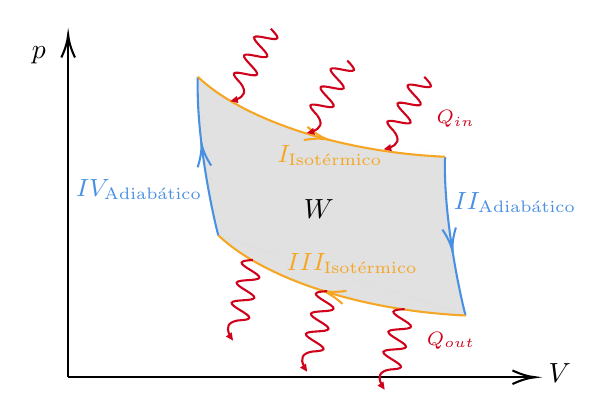
\begin{tikzpicture}[x=0.75pt,y=0.75pt,yscale=-1,xscale=1]
		%uncomment if require: \path (0,300); %set diagram left start at 0, and has height of 300
		
		%Shape: Parallelogram [id:dp9741257468547724] 
		\draw  [draw opacity=0][fill={rgb, 255:red, 155; green, 155; blue, 155 }  ,fill opacity=0.3 ] (92.5,40.5) -- (210.79,78.6) -- (220.89,155.07) -- (102.38,116.7) -- cycle ;
		%Curve Lines [id:da7911359963889097] 
		\draw [color={rgb, 255:red, 74; green, 144; blue, 226 }  ,draw opacity=1 ][fill={rgb, 255:red, 155; green, 155; blue, 155 }  ,fill opacity=0.3 ]   (102.38,116.71) .. controls (100.72,111.11) and (91.47,70.83) .. (92.46,40.25) ;
		\draw [shift={(94.24,72.58)}, rotate = 82.59] [color={rgb, 255:red, 74; green, 144; blue, 226 }  ,draw opacity=1 ][line width=0.75]    (10.93,-3.29) .. controls (6.95,-1.4) and (3.31,-0.3) .. (0,0) .. controls (3.31,0.3) and (6.95,1.4) .. (10.93,3.29)   ;
		%Curve Lines [id:da6573892726714319] 
		\draw [color={rgb, 255:red, 74; green, 144; blue, 226 }  ,draw opacity=1 ][fill={rgb, 255:red, 255; green, 255; blue, 255 }  ,fill opacity=1 ]   (221.5,155.25) .. controls (219.85,149.64) and (210.59,109.37) .. (211.58,78.78) ;
		\draw [shift={(215.19,124.17)}, rotate = 261.45] [color={rgb, 255:red, 74; green, 144; blue, 226 }  ,draw opacity=1 ][line width=0.75]    (10.93,-3.29) .. controls (6.95,-1.4) and (3.31,-0.3) .. (0,0) .. controls (3.31,0.3) and (6.95,1.4) .. (10.93,3.29)   ;
		%Curve Lines [id:da6114330108418855] 
		\draw [color={rgb, 255:red, 245; green, 166; blue, 35 }  ,draw opacity=1 ][fill={rgb, 255:red, 155; green, 155; blue, 155 }  ,fill opacity=0.3 ]   (102.46,116.71) .. controls (123.95,137.1) and (170.25,152.91) .. (221.5,155.25) ;
		\draw [shift={(152.69,143.35)}, rotate = 16.91] [color={rgb, 255:red, 245; green, 166; blue, 35 }  ,draw opacity=1 ][line width=0.75]    (10.93,-3.29) .. controls (6.95,-1.4) and (3.31,-0.3) .. (0,0) .. controls (3.31,0.3) and (6.95,1.4) .. (10.93,3.29)   ;
		%Curve Lines [id:da8532109473148837] 
		\draw [color={rgb, 255:red, 245; green, 166; blue, 35 }  ,draw opacity=1 ][fill={rgb, 255:red, 255; green, 255; blue, 255 }  ,fill opacity=1 ]   (92.46,40.25) .. controls (113.95,60.64) and (160.25,76.44) .. (211.5,78.78) ;
		\draw [shift={(154.97,70.43)}, rotate = 195.25] [color={rgb, 255:red, 245; green, 166; blue, 35 }  ,draw opacity=1 ][line width=0.75]    (10.93,-3.29) .. controls (6.95,-1.4) and (3.31,-0.3) .. (0,0) .. controls (3.31,0.3) and (6.95,1.4) .. (10.93,3.29)   ;
		
		%Shape: Wave [id:dp39168695581197555] 
		\draw  [color={rgb, 255:red, 208; green, 2; blue, 27 }  ,draw opacity=1 ] (154.81,143.51) .. controls (152.13,143.69) and (149.58,143.86) .. (149.36,144.73) .. controls (149.14,145.61) and (151.32,146.96) .. (153.61,148.37) .. controls (155.9,149.77) and (158.08,151.12) .. (157.86,152) .. controls (157.64,152.88) and (155.09,153.04) .. (152.4,153.22) .. controls (149.72,153.39) and (147.17,153.56) .. (146.95,154.44) .. controls (146.73,155.32) and (148.91,156.66) .. (151.2,158.07) .. controls (153.49,159.48) and (155.67,160.82) .. (155.45,161.7) .. controls (155.23,162.58) and (152.68,162.75) .. (149.99,162.92) .. controls (147.31,163.1) and (144.76,163.27) .. (144.54,164.14) .. controls (144.32,165.02) and (146.5,166.37) .. (148.79,167.78) .. controls (151.08,169.18) and (153.26,170.53) .. (153.04,171.41) .. controls (152.82,172.29) and (150.26,172.45) .. (147.58,172.63) ;
		%Curve Lines [id:da3709175237204154] 
		\draw [color={rgb, 255:red, 208; green, 2; blue, 27 }  ,draw opacity=1 ]   (147.58,172.63) .. controls (142.55,173.5) and (141.78,176.02) .. (143.64,179.78) ;
		\draw [shift={(145.17,182.33)}, rotate = 235.71] [fill={rgb, 255:red, 208; green, 2; blue, 27 }  ,fill opacity=1 ][line width=0.08]  [draw opacity=0] (3.57,-1.72) -- (0,0) -- (3.57,1.72) -- cycle    ;
		
		%Shape: Wave [id:dp1691880955779308] 
		\draw  [color={rgb, 255:red, 208; green, 2; blue, 27 }  ,draw opacity=1 ] (119.06,128.51) .. controls (116.38,128.69) and (113.82,128.86) .. (113.6,129.73) .. controls (113.39,130.61) and (115.57,131.96) .. (117.85,133.37) .. controls (120.14,134.77) and (122.32,136.12) .. (122.1,137) .. controls (121.89,137.88) and (119.33,138.04) .. (116.65,138.22) .. controls (113.97,138.39) and (111.41,138.56) .. (111.19,139.44) .. controls (110.98,140.32) and (113.15,141.66) .. (115.44,143.07) .. controls (117.73,144.48) and (119.91,145.82) .. (119.69,146.7) .. controls (119.48,147.58) and (116.92,147.75) .. (114.24,147.92) .. controls (111.56,148.1) and (109,148.27) .. (108.78,149.14) .. controls (108.57,150.02) and (110.74,151.37) .. (113.03,152.78) .. controls (115.32,154.18) and (117.5,155.53) .. (117.28,156.41) .. controls (117.06,157.29) and (114.51,157.45) .. (111.83,157.63) ;
		%Curve Lines [id:da6961722383949592] 
		\draw [color={rgb, 255:red, 208; green, 2; blue, 27 }  ,draw opacity=1 ]   (111.83,157.63) .. controls (106.79,158.5) and (106.03,161.02) .. (107.89,164.78) ;
		\draw [shift={(109.42,167.33)}, rotate = 235.71] [fill={rgb, 255:red, 208; green, 2; blue, 27 }  ,fill opacity=1 ][line width=0.08]  [draw opacity=0] (3.57,-1.72) -- (0,0) -- (3.57,1.72) -- cycle    ;
		
		%Straight Lines [id:da44896074985643397] 
		\draw    (30,185) -- (253,185) ;
		\draw [shift={(255,185)}, rotate = 180] [color={rgb, 255:red, 0; green, 0; blue, 0 }  ][line width=0.75]    (10.93,-3.29) .. controls (6.95,-1.4) and (3.31,-0.3) .. (0,0) .. controls (3.31,0.3) and (6.95,1.4) .. (10.93,3.29)   ;
		%Straight Lines [id:da035788672304859714] 
		\draw    (30,185) -- (30,22) ;
		\draw [shift={(30,20)}, rotate = 90] [color={rgb, 255:red, 0; green, 0; blue, 0 }  ][line width=0.75]    (10.93,-3.29) .. controls (6.95,-1.4) and (3.31,-0.3) .. (0,0) .. controls (3.31,0.3) and (6.95,1.4) .. (10.93,3.29)   ;
		%Shape: Wave [id:dp5008708149061333] 
		\draw  [color={rgb, 255:red, 208; green, 2; blue, 27 }  ,draw opacity=1 ] (192.15,152.18) .. controls (189.47,152.35) and (186.91,152.52) .. (186.69,153.4) .. controls (186.47,154.28) and (188.65,155.62) .. (190.94,157.03) .. controls (193.23,158.44) and (195.41,159.79) .. (195.19,160.66) .. controls (194.97,161.54) and (192.42,161.71) .. (189.74,161.88) .. controls (187.05,162.06) and (184.5,162.23) .. (184.28,163.11) .. controls (184.06,163.98) and (186.24,165.33) .. (188.53,166.74) .. controls (190.82,168.15) and (193,169.49) .. (192.78,170.37) .. controls (192.56,171.25) and (190.01,171.42) .. (187.33,171.59) .. controls (184.64,171.76) and (182.09,171.93) .. (181.87,172.81) .. controls (181.65,173.69) and (183.83,175.03) .. (186.12,176.44) .. controls (188.41,177.85) and (190.59,179.2) .. (190.37,180.07) .. controls (190.15,180.95) and (187.6,181.12) .. (184.92,181.29) ;
		%Curve Lines [id:da14005587645379003] 
		\draw [color={rgb, 255:red, 208; green, 2; blue, 27 }  ,draw opacity=1 ]   (184.92,181.29) .. controls (179.88,182.17) and (179.11,184.69) .. (180.98,188.45) ;
		\draw [shift={(182.5,191)}, rotate = 235.71] [fill={rgb, 255:red, 208; green, 2; blue, 27 }  ,fill opacity=1 ][line width=0.08]  [draw opacity=0] (3.57,-1.72) -- (0,0) -- (3.57,1.72) -- cycle    ;
		
		%Shape: Wave [id:dp9642837331485368] 
		\draw  [color={rgb, 255:red, 208; green, 2; blue, 27 }  ,draw opacity=1 ] (164.5,32.42) .. controls (166.33,34.37) and (168.07,36.23) .. (167.63,37.02) .. controls (167.18,37.81) and (164.68,37.31) .. (162.06,36.79) .. controls (159.44,36.26) and (156.93,35.77) .. (156.49,36.56) .. controls (156.05,37.35) and (157.79,39.2) .. (159.62,41.15) .. controls (161.45,43.1) and (163.19,44.95) .. (162.75,45.74) .. controls (162.31,46.53) and (159.81,46.04) .. (157.19,45.51) .. controls (154.56,44.99) and (152.06,44.5) .. (151.62,45.28) .. controls (151.18,46.07) and (152.92,47.93) .. (154.75,49.88) .. controls (156.58,51.83) and (158.32,53.68) .. (157.88,54.47) .. controls (157.44,55.26) and (154.94,54.77) .. (152.31,54.24) .. controls (149.69,53.72) and (147.19,53.22) .. (146.75,54.01) .. controls (146.3,54.8) and (148.05,56.66) .. (149.87,58.61) ;
		%Curve Lines [id:da6832608000261728] 
		\draw [color={rgb, 255:red, 208; green, 2; blue, 27 }  ,draw opacity=1 ]   (149.87,58.61) .. controls (152.93,62.66) and (151.77,65.02) .. (147.85,66.5) ;
		\draw [shift={(145,67.33)}, rotate = 347.17] [fill={rgb, 255:red, 208; green, 2; blue, 27 }  ,fill opacity=1 ][line width=0.08]  [draw opacity=0] (3.57,-1.72) -- (0,0) -- (3.57,1.72) -- cycle    ;
		
		%Shape: Wave [id:dp2902956876051962] 
		\draw  [color={rgb, 255:red, 208; green, 2; blue, 27 }  ,draw opacity=1 ] (201.58,40.26) .. controls (203.41,42.2) and (205.15,44.06) .. (204.71,44.85) .. controls (204.27,45.64) and (201.77,45.14) .. (199.14,44.62) .. controls (196.52,44.1) and (194.02,43.6) .. (193.58,44.39) .. controls (193.14,45.18) and (194.88,47.04) .. (196.71,48.98) .. controls (198.54,50.93) and (200.28,52.79) .. (199.83,53.58) .. controls (199.39,54.37) and (196.89,53.87) .. (194.27,53.35) .. controls (191.64,52.82) and (189.14,52.33) .. (188.7,53.12) .. controls (188.26,53.91) and (190,55.76) .. (191.83,57.71) .. controls (193.66,59.66) and (195.4,61.52) .. (194.96,62.31) .. controls (194.52,63.1) and (192.02,62.6) .. (189.4,62.08) .. controls (186.77,61.55) and (184.27,61.06) .. (183.83,61.85) .. controls (183.39,62.64) and (185.13,64.49) .. (186.96,66.44) ;
		%Curve Lines [id:da5127770232418957] 
		\draw [color={rgb, 255:red, 208; green, 2; blue, 27 }  ,draw opacity=1 ]   (186.96,66.44) .. controls (190.02,70.49) and (188.85,72.85) .. (184.94,74.34) ;
		\draw [shift={(182.08,75.17)}, rotate = 347.17] [fill={rgb, 255:red, 208; green, 2; blue, 27 }  ,fill opacity=1 ][line width=0.08]  [draw opacity=0] (3.57,-1.72) -- (0,0) -- (3.57,1.72) -- cycle    ;
		
		%Shape: Wave [id:dp6039569178637453] 
		\draw  [color={rgb, 255:red, 208; green, 2; blue, 27 }  ,draw opacity=1 ] (127.65,17.08) .. controls (129.48,19.03) and (131.22,20.88) .. (130.78,21.67) .. controls (130.34,22.46) and (127.84,21.97) .. (125.22,21.44) .. controls (122.59,20.92) and (120.09,20.42) .. (119.65,21.21) .. controls (119.21,22) and (120.95,23.86) .. (122.78,25.81) .. controls (124.61,27.75) and (126.35,29.61) .. (125.91,30.4) .. controls (125.47,31.19) and (122.97,30.69) .. (120.34,30.17) .. controls (117.72,29.65) and (115.22,29.15) .. (114.78,29.94) .. controls (114.33,30.73) and (116.08,32.59) .. (117.9,34.53) .. controls (119.73,36.48) and (121.47,38.34) .. (121.03,39.13) .. controls (120.59,39.92) and (118.09,39.42) .. (115.47,38.9) .. controls (112.84,38.37) and (110.34,37.88) .. (109.9,38.67) .. controls (109.46,39.46) and (111.2,41.32) .. (113.03,43.26) ;
		%Curve Lines [id:da27385014219912984] 
		\draw [color={rgb, 255:red, 208; green, 2; blue, 27 }  ,draw opacity=1 ]   (113.03,43.26) .. controls (116.09,47.32) and (114.93,49.68) .. (111.01,51.16) ;
		\draw [shift={(108.16,51.99)}, rotate = 347.17] [fill={rgb, 255:red, 208; green, 2; blue, 27 }  ,fill opacity=1 ][line width=0.08]  [draw opacity=0] (3.57,-1.72) -- (0,0) -- (3.57,1.72) -- cycle    ;
		
		
		% Text Node
		\draw (260,177) node [anchor=north west][inner sep=0.75pt]   [align=left] {$\displaystyle V$};
		% Text Node
		\draw (11,24) node [anchor=north west][inner sep=0.75pt]   [align=left] {$\displaystyle p$};
		% Text Node
		\draw (129.33,71.67) node [anchor=north west][inner sep=0.75pt]  [font=\small,color={rgb, 255:red, 245; green, 166; blue, 35 }  ,opacity=1 ] [align=left] {$\displaystyle I_{\text{Isotérmico}}$};
		% Text Node
		\draw (133.71,124) node [anchor=north west][inner sep=0.75pt]  [font=\small,color={rgb, 255:red, 245; green, 166; blue, 35 }  ,opacity=1 ] [align=left] {$\displaystyle III_{\text{Isotérmico}}$};
		% Text Node
		\draw (214.33,94.67) node [anchor=north west][inner sep=0.75pt]  [font=\small,color={rgb, 255:red, 74; green, 144; blue, 226 }  ,opacity=1 ] [align=left] {$\displaystyle II_{\text{Adiabático}}$};
		% Text Node
		\draw (32.33,88.33) node [anchor=north west][inner sep=0.75pt]  [font=\small,color={rgb, 255:red, 74; green, 144; blue, 226 }  ,opacity=1 ] [align=left] {$\displaystyle IV_{\text{Adiabático}}$};
		% Text Node
		\draw (206,55) node [anchor=north west][inner sep=0.75pt]  [font=\scriptsize,color={rgb, 255:red, 208; green, 2; blue, 27 }  ,opacity=1 ] [align=left] {$\displaystyle Q_{in}$};
		% Text Node
		\draw (201.33,161.67) node [anchor=north west][inner sep=0.75pt]  [font=\scriptsize,color={rgb, 255:red, 208; green, 2; blue, 27 }  ,opacity=1 ] [align=left] {$\displaystyle Q_{out}$};
		% Text Node
		\draw (142.13,98) node [anchor=north west][inner sep=0.75pt]   [align=left] {$\displaystyle W$};
	\end{tikzpicture}
\end{figure}

\subsection{Segunda ley}
\caja{Entropía ($S$)}{Cuantifica la irreversibilidad, es una variable de estado que indica la dirección en la que ocurre un proceso irreversible.}

La entropía de un sistema aislado incrementa o se mantiene constante ante cualquier proceso espontaneo y natural, manteniéndose constante solo frente a procesos reversibles.
\begin{equation}
	\Delta S \geq 0
\end{equation}

\subsubsection{Variables intensivas y extensivas}
\begin{itemize}
	\item Variable intensiva: Independiente del tamaño del sistema (presión, temperatura, densidad, conductividad).
	\item Variable extensiva: Crece proporcional al tamaño del sistema (volumen, número de partículas, masa, energía interna).
\end{itemize}

\subsubsection{Entropía}
La entropía es una variable extensiva (crece con el tamaño). Un sistema formado por $n$ subsistemas tendrá una entropía:
\begin{equation}
	S=\sum_{i}^{n}S_i
\end{equation}

\caja{Reservorio de calor}{Sistema ideal infinitamente grande a $T$ constante y capacidad calórica infinita, es decir, $T$ no cambia cuando el depósito absorbe o entrega calor.}
\caja{Eficiencia termodinámica ($\eta$)}{Razón entre trabajo realizado por un sistema termodinámico y el calor que se le entrega. \[\eta=\frac{W_{out}}{Q_{in}}\]}

Si tenemos una máquina de Carnot entre dos reservorios a distintas temperaturas $T_H$ y $T_C$, donde $T_H>T_C$, el sistema extraerá calor $Q_H$ del reservorio a mayor temperatura $T_H$, realizará un trabajo $W$, y liberará calor $Q_C$ reservorio frío $T_C$.
\begin{figure}[h!]
	\centering
	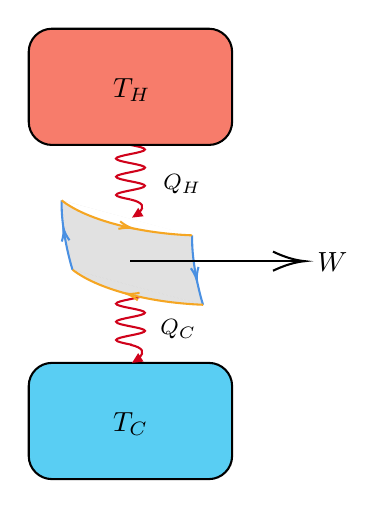
\begin{tikzpicture}[x=0.75pt,y=0.75pt,yscale=-1.4,xscale=1.4]
		%Rounded Rect [id:dp01756133045023911] 
		\draw  [fill={rgb, 255:red, 89; green, 206; blue, 243 }  ,fill opacity=1 ] (30,143) .. controls (30,138.58) and (33.58,135) .. (38,135) -- (92,135) .. controls (96.42,135) and (100,138.58) .. (100,143) -- (100,167) .. controls (100,171.42) and (96.42,175) .. (92,175) -- (38,175) .. controls (33.58,175) and (30,171.42) .. (30,167) -- cycle ;
		%Shape: Wave [id:dp8415707433965373] 
		\draw  [color={rgb, 255:red, 208; green, 2; blue, 27 }  ,draw opacity=1 ] (68.43,112.29) .. controls (67.51,112.55) and (66.28,112.8) .. (65.03,113.05) .. controls (62.48,113.56) and (60.06,114.06) .. (60.06,114.62) .. controls (60.06,115.19) and (62.48,115.67) .. (65.03,116.18) .. controls (67.58,116.68) and (70,117.16) .. (70,117.73) .. controls (70,118.3) and (67.58,118.79) .. (65.03,119.3) .. controls (62.48,119.82) and (60.06,120.31) .. (60.06,120.87) .. controls (60.06,121.44) and (62.48,121.92) .. (65.03,122.43) .. controls (67.58,122.93) and (70,123.42) .. (70,123.98) .. controls (70,124.55) and (67.58,125.04) .. (65.03,125.55) .. controls (62.48,126.07) and (60.06,126.56) .. (60.06,127.12) .. controls (60.06,127.69) and (62.48,128.17) .. (65.03,128.68) .. controls (65.16,128.71) and (65.29,128.73) .. (65.43,128.76) ;
		%Curve Lines [id:da34181029196406476] 
		\draw [color={rgb, 255:red, 208; green, 2; blue, 27 }  ,draw opacity=1 ]   (65,128.76) .. controls (69.47,129.81) and (69.99,131.31) .. (67.95,133.23) ;
		\draw [shift={(65.57,135)}, rotate = 327.74] [fill={rgb, 255:red, 208; green, 2; blue, 27 }  ,fill opacity=1 ][line width=0.08]  [draw opacity=0] (3.57,-1.72) -- (0,0) -- (3.57,1.72) -- cycle    ;
		%Shape: Parallelogram [id:dp9033291024670296] 
		\draw  [draw opacity=0][fill={rgb, 255:red, 155; green, 155; blue, 155 }  ,fill opacity=0.3 ] (41.35,79.05) -- (85.96,91.2) -- (89.77,114.93) -- (45.09,102.96) -- cycle ;
		%Curve Lines [id:da2928516850674865] 
		\draw [color={rgb, 255:red, 74; green, 144; blue, 226 }  ,draw opacity=1 ][fill={rgb, 255:red, 155; green, 155; blue, 155 }  ,fill opacity=0.3 ]   (45.09,102.96) .. controls (44.47,101.21) and (40.97,88.63) .. (41.35,79.08) ;
		\draw [shift={(41.96,88.72)}, rotate = 80.14] [color={rgb, 255:red, 74; green, 144; blue, 226 }  ,draw opacity=1 ][line width=0.75]    (4.37,-1.32) .. controls (2.78,-0.56) and (1.32,-0.12) .. (0,0) .. controls (1.32,0.12) and (2.78,0.56) .. (4.37,1.32)   ;
		%Curve Lines [id:da1357732366419231] 
		\draw [color={rgb, 255:red, 74; green, 144; blue, 226 }  ,draw opacity=1 ][fill={rgb, 255:red, 255; green, 255; blue, 255 }  ,fill opacity=1 ]   (90,115) .. controls (89.38,113.25) and (85.89,100.67) .. (86.26,91.11) ;
		\draw [shift={(87.86,106.53)}, rotate = 260.23] [color={rgb, 255:red, 74; green, 144; blue, 226 }  ,draw opacity=1 ][line width=0.75]    (4.37,-1.32) .. controls (2.78,-0.56) and (1.32,-0.12) .. (0,0) .. controls (1.32,0.12) and (2.78,0.56) .. (4.37,1.32)   ;
		%Curve Lines [id:da8502156589832992] 
		\draw [color={rgb, 255:red, 245; green, 166; blue, 35 }  ,draw opacity=1 ][fill={rgb, 255:red, 155; green, 155; blue, 155 }  ,fill opacity=0.3 ]   (45.12,102.96) .. controls (53.22,109.33) and (70.68,114.27) .. (90,115) ;
		\draw [shift={(63.59,111.16)}, rotate = 13.35] [color={rgb, 255:red, 245; green, 166; blue, 35 }  ,draw opacity=1 ][line width=0.75]    (4.37,-1.32) .. controls (2.78,-0.56) and (1.32,-0.12) .. (0,0) .. controls (1.32,0.12) and (2.78,0.56) .. (4.37,1.32)   ;
		%Curve Lines [id:da07790949040581341] 
		\draw [color={rgb, 255:red, 245; green, 166; blue, 35 }  ,draw opacity=1 ][fill={rgb, 255:red, 255; green, 255; blue, 255 }  ,fill opacity=1 ]   (41.35,79.08) .. controls (49.45,85.45) and (66.91,90.38) .. (86.23,91.11) ;
		\draw [shift={(65.42,88.61)}, rotate = 193.49] [color={rgb, 255:red, 245; green, 166; blue, 35 }  ,draw opacity=1 ][line width=0.75]    (4.37,-1.32) .. controls (2.78,-0.56) and (1.32,-0.12) .. (0,0) .. controls (1.32,0.12) and (2.78,0.56) .. (4.37,1.32)   ;
		
		%Straight Lines [id:da872698874734591] 
		\draw    (65,100) -- (123,100) ;
		\draw [shift={(125,100)}, rotate = 180] [color={rgb, 255:red, 0; green, 0; blue, 0 }  ][line width=0.75]    (10.93,-3.29) .. controls (6.95,-1.4) and (3.31,-0.3) .. (0,0) .. controls (3.31,0.3) and (6.95,1.4) .. (10.93,3.29)   ;
		%Shape: Wave [id:dp46606163354074404] 
		\draw  [color={rgb, 255:red, 208; green, 2; blue, 27 }  ,draw opacity=1 ] (65.03,60) .. controls (67.58,60.51) and (70,60.99) .. (70,61.56) .. controls (70,62.12) and (67.58,62.62) .. (65.03,63.13) .. controls (62.48,63.64) and (60.06,64.14) .. (60.06,64.7) .. controls (60.06,65.27) and (62.48,65.75) .. (65.03,66.26) .. controls (67.58,66.76) and (70,67.24) .. (70,67.81) .. controls (70,68.38) and (67.58,68.87) .. (65.03,69.38) .. controls (62.48,69.9) and (60.06,70.39) .. (60.06,70.95) .. controls (60.06,71.52) and (62.48,72) .. (65.03,72.51) .. controls (67.58,73.01) and (70,73.5) .. (70,74.06) .. controls (70,74.63) and (67.58,75.12) .. (65.03,75.63) .. controls (62.48,76.15) and (60.06,76.64) .. (60.06,77.2) .. controls (60.06,77.77) and (62.48,78.25) .. (65.03,78.76) ;
		%Curve Lines [id:da3854672887405194] 
		\draw [color={rgb, 255:red, 208; green, 2; blue, 27 }  ,draw opacity=1 ]   (65,78.76) .. controls (69.47,79.81) and (69.99,81.31) .. (67.95,83.23) ;
		\draw [shift={(65.57,85)}, rotate = 327.74] [fill={rgb, 255:red, 208; green, 2; blue, 27 }  ,fill opacity=1 ][line width=0.08]  [draw opacity=0] (3.57,-1.72) -- (0,0) -- (3.57,1.72) -- cycle    ;
		
		%Rounded Rect [id:dp10591783414821498] 
		\draw  [fill={rgb, 255:red, 247; green, 124; blue, 107 }  ,fill opacity=1 ] (30,28) .. controls (30,23.58) and (33.58,20) .. (38,20) -- (92,20) .. controls (96.42,20) and (100,23.58) .. (100,28) -- (100,52) .. controls (100,56.42) and (96.42,60) .. (92,60) -- (38,60) .. controls (33.58,60) and (30,56.42) .. (30,52) -- cycle ;
		
		% Text Node
		\draw (58,36) node [anchor=north west][inner sep=0.75pt]   [align=left] {$\displaystyle T_{H}$};
		% Text Node
		\draw (58,151) node [anchor=north west][inner sep=0.75pt]   [align=left] {$\displaystyle T_{C}$};
		% Text Node
		\draw (75.25,69) node [anchor=north west][inner sep=0.75pt]  [font=\footnotesize] [align=left] {$\displaystyle Q_{H}$};
		% Text Node
		\draw (74.25,119) node [anchor=north west][inner sep=0.75pt]  [font=\footnotesize] [align=left] {$\displaystyle Q_{C}$};
		% Text Node
		\draw (128.25,96) node [anchor=north west][inner sep=0.75pt]   [align=left] {$\displaystyle W$};
	\end{tikzpicture}
\end{figure}

En el caso de una máquina de Carnot ideal tendremos que:
\begin{align}
	\eta &= \frac{W_{out}}{Q_{in}} = 1-\frac{Q_C}{Q_H}\nonumber\\
	&= 1-\frac{T_C}{T_H}
\end{align}
\begin{equation}
	dS=\frac{\delta Q}{T}
\end{equation}
El caso general, incluyendo procesos irreversibles, tendremos la desigualdad 
\begin{equation}
	dS\geq\frac{\delta Q}{T}
\end{equation}
Ya que, el trabajo realizado sobre un sistema será mayor en el caso irreversible ($\delta W_{\text{irr}}>\delta W_{\text{rev}}$). Es decir, al ejercer trabajo irreversible parte de la energía se disipa en energía interna (ya sea fricción, turbulencia, etc.), resultando en un aumento de entropía.

\subsubsection{Ecuación fundamental}
En un caso reversible, podemos escribir la primera ley para un sistema en equilibrio como
\begin{align}
	dE &= \delta Q + \delta W \left\lbrace \begin{matrix}
		\delta W = -p dV\\
		\delta Q = T dS
	\end{matrix}\right.\nonumber\\
	\therefore dE &= TdS - pdV
	\label{eqn:fund_eqn}
\end{align}
Este es el caso más sencillo donde el trabajo solo depende del volumen del cuerpo, pero sistemas más complejos pueden incluir términos de tensión superficial, campo magnético, etc.

Recordando la definición de diferencial exacto en la ecuación \ref{eqn:def_dif_exacto}, podemos escribir las equivalencias
\begin{align}
	T = &\left(\frac{\partial E}{\partial S}\right)_V\\
	p = -&\left(\frac{\partial E}{\partial V}\right)_S
\end{align}

\subsubsection{Relaciones de Maxwell}
Debido a las ecuaciones \ref{eqn:orden_dif} y \ref{eqn:orden_dif2}, las derivadas cruzadas deben ser iguales:
\begin{align}
	\frac{\partial^2E}{\partial S\partial V} &= \frac{\partial^2E}{\partial V\partial S}\nonumber\\
	\Rightarrow \left(\frac{\partial T}{\partial V}\right)_S &= -\left(\frac{\partial p}{\partial S}\right)_V \label{eqn:maxwell_rel1}
\end{align}
Pero escribir $E=E(S,V)$ es complicado, porque es difícil variar $S$ desde un laboratorio.

Con un poco de álgebra podemos transformar \ref{eqn:fund_eqn} en:
\begin{equation}
	dS = \frac{1}{T}dE + \frac{p}{T}dV,
\end{equation}
lo cual hace $dS=dS(E,V)$. Y, de nuevo por la definición de diferencial exacto (ecuación \ref{eqn:def_dif_exacto}), llegamos a:
\begin{align}
	\frac{1}{T} &= \left(\frac{\partial S}{\partial E}\right)_V\\
	\frac{p}{T} &= \left(\frac{\partial S}{\partial V}\right)_E
\end{align}

Y la relación de Maxwell:
\begin{align}
	\frac{\partial^2S}{\partial E\partial V} &= \frac{\partial^2S}{\partial V\partial E}\nonumber\\
	\Rightarrow \left( \frac{\partial}{\partial E}\left(\frac{\partial S}{\partial V}\right)_E\right)_V &= \left( \frac{\partial}{\partial V}\left(\frac{\partial S}{\partial E}\right)_V\right)_E \nonumber\\
	\Rightarrow \left( \frac{\partial}{\partial E}\left(\frac{1}{T}\right)\right)_V &= \left( \frac{\partial}{\partial V}\left(\frac{p}{T}\right)\right)_E \label{eqn:maxwell_rel2}
\end{align}

\subsection{Tercera Ley}
La entropía tiende a un valor fijo, independiente de las variables de estado cuando la temperatura tiende a cero absoluto.

Esta ley sólo se puede demostrar en teoría cuántica. En termodinámica clásica no nos interesa, puesto que sólo nos importan las diferencias de entropía y no sus valores absolutos.

\begin{equation}
	\lim_{T\rightarrow0}S = 0
\end{equation}

\subsection{Potenciales termodinámicos}
Para un sistema que puede cambiar su cantidad de partículas tendremos la siguiente ecuación fundamental:
\begin{equation}
	dE = TdS - pdV + \mu dN,
\end{equation}
donde $\mu$ es el potencial químico y $N$ la cantidad de partículas. Por lo que $E = E(S,V,N)$ y
\begin{equation}
	dE =  \underbrace{\left(\frac{\partial E}{\partial S}\right)_{V,N}}_{T}dS + \underbrace{\left(\frac{\partial E}{\partial V}\right)_{S,N}}_{-p}dV + \underbrace{\left(\frac{\partial E}{\partial N}\right)_{S,V}}_{\mu}dN
\end{equation}
y relaciones de Maxwell
\begin{alignat}{2}
	\deriv{T}{V}{S,N}   &= - &&\deriv{p  }{S}{V,N}\\
	\deriv{T}{N}{S,V}   &= \ &&\deriv{\mu}{S}{V,N}\\
	\deriv{\mu}{V}{S,N} &= - &&\deriv{p  }{N}{S,V}
\end{alignat}

Pero es más práctico trabajar con $S=S(E,V,N)$, porque experimentalmente en un sistema aislado se ajusta $(E,V,V)$. Tenemos entonces
\begin{equation}
	dS = \frac{1}{T}dE + \frac{p}{T} - \frac{\mu}{T}dN
\end{equation}
por ende
\begin{equation}
	\begin{matrix}
		\dderiv{S}{E}{V,N} =  \dfrac{1}{T},\ \ \ & \dderiv{S}{V}{E,N} =  \dfrac{p}{T},\ \ \ & \dderiv{S}{N}{E,V} = -\dfrac{\mu}{T}
	\end{matrix}
\end{equation}

En un sistema aislado las variables $(E,V,N)$ son fijas. Cualquier otra variable interna se ajusta al valor donde la entropía sea máxima.

\subsubsection{Energía libre de Helmholtz}
Para sistemas con T fijada externamente, es más práctico usar $(T,V,N)$.

Sabemos que \(\dderiv{E}{V}{S} = -p\), por lo que a partir de la ecuación \ref{eqn:fund_eqn}\footnote{\(dE = \dderiv{E}{S}{V}dS + \dderiv{E}{V}{S}dV \Rightarrow \dderiv{E}{V}{T} = \dderiv{E}{S}{V} \dderiv{S}{V}{T} + \dderiv{E}{V}{S}\cancel{\dderiv{V}{V}{T}}\)}:
\begin{align}
	\deriv{E}{V}{T} = \underbrace{\deriv{E}{V}{S}}_{-p} + \underbrace{\deriv{E}{S}{V}}_{T}\deriv{S}{V}{T}\nonumber\\
	\Rightarrow\deriv{}{V}{T}(E-TS) = -p
\end{align}

Por otro lado, usando regla de la cadena
\begin{align}
	\deriv{E}{T}{V} &= \deriv{E}{S}{V}\deriv{S}{T}{V}\nonumber\\
	&= T\deriv{S}{T}{V} = \deriv{(TS)}{T}{V} - S\nonumber\\
	\Rightarrow\deriv{}{T}{V}(E-TS) &= -S
\end{align}

Ahora podemos definir
\begin{equation}
	F \equiv E-TS,
\end{equation}
donde $F=F(T,V,N)$ es la \textbf{energía libre de Helmholtz}. Se cumple además que:
\begin{align}
	\deriv{F}{T}{V} &= -S\\
	\deriv{F}{V}{T} &= -p
\end{align}
su diferencial:
\begin{equation}
	dF = -SdT - pdV + \mu dN
\end{equation}
y derivadas parciales:
\begin{equation}
	\begin{matrix}
		\dderiv{F}{T}{V,N} = -S,\ \ \ & \dderiv{F}{V}{T,N} = -p,\ \ \ & \dderiv{F}{N}{T,V} = \mu
	\end{matrix}
\end{equation}

Conceptualmente, \(F\) representa la máxima energía disponible por un sistema para ejercer trabajo sobre el exterior.
%\subsubsection{Transformadas de Legendre}

\subsubsection{Calores específicos}
\caja{Calor específico parte 2}{Podemos definir varias versiones del calor específico, las dos que más nos importan son el calor específico a volumen constante (\(c_V\)) y a presión constante (\(c_p\)), definidos matemáticamente como: \[c_V=\dderiv{E}{T}{V},\ \ \ c_p=\dderiv{E}{T}{p}\]}

Asumimos un tanque rígido (\(V\) constante \(\Leftrightarrow dV=0\)) lleno de un gas al que le aplicamos una pequeña cantidad de calor \(\delta Q\). El trabajo realizado sobre el sistema será \(\delta W = pdV = 0\), luego, por la primera ley: \(dE = \delta Q + 0\). Ya que el calor específico \(c_V\) se define como el calor necesario para elevar en una unidad la temperatura de una molécula, la fórmula del calor agregado al sistema será: \(\delta Q = N c_V dT\), por lo que:
\begin{equation*}
	dE = N c_V dT
\end{equation*}
e integrando:
\begin{equation}
	E = N c_V T
\end{equation}

Considerando ahora un sistema similar pero con el gas de un pistón que puede moverse libremente, tendremos que \(dV\neq 0\) y \(p\) constante. Añadimos de nuevo un calor \(\delta Q = N c_p dT\), mientras que el trabajo ejercido por el sistema será \(\delta Q = -p dV\) (negativo porque es trabajo ejercido \textit{por} el sistema sobre el universo). Tendremos entonces:
\begin{equation*}
	dE = N c_p dT - p dV
\end{equation*}
Tomando la ecuación \ref{eqn:gases_ideales} de gases ideales (\(pV = NkT\)) si la presión es constante:
\begin{equation*}
	p dV = Nk dT
\end{equation*}
Y sustituyendo de vuelta en la ecuación:
\begin{equation*}
	dE = N (c_p-k) dT
\end{equation*}
Y, ya que la energía es una función de estado y un diferencial exacto, \(dE\) será independiente del camino que tomamos para elevar la temperatura, por lo que podemos igualar ambas ecuaciones para \(dE\):
\begin{align}
	N c_V dT &= N (c_p-k) dT\nonumber\\
	c_p &= c_V + k
\end{align}

\subsubsection{Helmholtz y entropía para un gas ideal}
Saltándome toda la derivación, se puede llegar a que las expresiones de la energía libre de Helmholtz y de la entropía para un gas ideal:
\begin{align}
	F(T,V) &= -Nc_VT\ln\frac{T}{T_0} - NkT\ln\frac{V}{V_0} + F_0\\
	S(T,V) &= Nc_pT\ln\frac{T}{T_0} + Nk\ln\frac{p}{p_0} + Ns_0
\end{align}
donde \(T_0, V_0, p_0, F_0, s_0\) son puntos de referencia arbitrarios (al hacer una diferencia \(\Delta S = S_2 - S_1\) deberían cancelarse, no pienses mucho en eso).

\subsubsection{Relación de Euler}
De la relación fundamental \(dE = TdS - pdV + \mu dN\) tenemos 4 variables extensivas \(E, S, V, N\) y 3 intensivas \(T, p, \mu\). Si el sistema crece homogéneamente por un factor \(\alpha\) tendremos:
\begin{equation*}
	E(S,V,N)\rightarrow E(\alpha S,\alpha V,\alpha N) = \alpha (S,V,N)
\end{equation*}
Derivando respecto a \(\alpha\) llegamos a la \textbf{relación de Euler}:
\begin{equation}
	E = TS - pV + \mu N
\end{equation}
Diferenciando obtenemos:
\begin{align*}
	dE &= SdT + TdS - Vdp - pdV + Nd\mu + \mu dN \nonumber\\
	dE &= (TdS - pdV + \mu dN) + SdT - Vdp + Nd\mu \nonumber\\
	dE &= (dE) + SdT - Vdp + Nd\mu \nonumber
\end{align*}
\begin{equation}\\
	\Rightarrow SdT - Vdp + Nd\mu = 0
\end{equation}
Considerando las variables extensivas que aparecen \(S,V,N\), de aquí concluimos un \textit{constraint} que limita a \textbf{dos} las variables intensivas e independientes.

Tomando el potencial químico \(\mu\) como ejemplo:
\begin{equation}
	d\mu = -sdT + vdp
\end{equation}
donde \(s=\dfrac{S}{N}, v=\dfrac{V}{N}\). Además para un gas ideal tenemos:
\begin{align*}
	v &= \frac{kT}{p}\\
	s &= c_pT\ln\frac{T}{T_0} + k\ln\frac{p}{p_0} + s_0\\
	\therefore d\mu &= -c_pT\ln\frac{T}{T_0}dT - k\ln\frac{p}{p_0}dT - s_0dT + \frac{kT}{p}dp
\end{align*}
Integrando y tomando \(\mu_0 = (c_p - s_0)T_0 = 0\) (porque es un valor de referencia arbitrario y hacemos lo que queremos con él), tenemos el potencial químico para un gas ideal:
\begin{equation}
	\mu (T,p) = -c_pT\ln\frac{T}{T_0} + kT\ln\frac{p}{p_0} + (c_p-s_0)T
	\label{eqn:mu_gas_ideal}
\end{equation}

\subsubsection{Entalpía (\(H\))}
Es un potencial útil cuando las variables de control (externas) son \((S, p, N)\), los cuales son usualmente procesos adiabáticos a presión fija.
\begin{align}
	H &\equiv E + pV\\
	dH(S,p,N) &= TdS + Vdp + \mu dN
\end{align}
\begin{equation}
	\begin{matrix}
		\dderiv{H}{S}{p,N} = T,\ \ \ & \dderiv{H}{p}{S,N} = V,\ \ \ & \dderiv{H}{N}{S,p} = \mu
	\end{matrix}
\end{equation}

\(H\) es mínima en equilibrio.

\subsubsection{Energía Libre de Gibbs (\(G\))}
Es un potencial útil cuando las variables de control (externas) son \((T, p, N)\).
\begin{align}
	G &\equiv E - TS + pV\\
	dG(T,p,N) &= -SdT + Vdp + \mu dN
\end{align}
\begin{equation}
	\begin{matrix}
		\dderiv{G}{T}{p,N} = -S,\ \ \ & \dderiv{G}{p}{T,N} = V,\ \ \ & \dderiv{G}{N}{T,p} = \mu
	\end{matrix}
\end{equation}

Notando que en \(G(T,p,N)\) la única variable extensiva es  \(N\), por lo que:
\begin{equation*}
	G(T,p,\alpha N) = \alpha G(T,p,N)
\end{equation*}
Derivando,
\begin{equation}
	G = \mu N
\end{equation}
Si la sustancia está compuesta por varios tipos de partículas, se cumplirá, en cambio, que
\begin{equation}
	G = \sum_{i}\mu_i N_i
	\label{eqn:Gibbs_suma_mu}
\end{equation}

También se cumple que
\begin{equation}
	H = -T^2 \deriv{(G/T)}{T}{p}
\end{equation}

\(G\) es mínima en equilibrio.

\subsection{Potencial Químico y Difusión}
El potencial químico es aquello que, en equilibrio, se iguala ante difusión de partículas de una región a otra. Intuitivamente, ocurre difusión cuando hay diferencia de concentración, pero en rigor es cuando hay \textbf{diferencia en el potencial químico}.

Un ejemplo es la atmósfera en equilibrio térmico, la temperatura debe ser igual en todas partes (atmósfera isotérmica) y el potencial químico debe ser igual en todas partes (la densidad debe cambiar con la altura). Tomando la expresión \ref{eqn:mu_gas_ideal}
\begin{equation*}
	\mu (T,p) = -c_pT\ln\frac{T}{T_0} + kT\ln\frac{p}{p_0} + (c_p-s_0)T
\end{equation*}
Y le agregamos el efecto de la energía potencial gravitatoria mediante la relación de Euler:
\begin{align*}
	E &= TS - pV + \mu N\\
	E = E_K &\rightarrow E = E_K + E_P\\
	E &= E_K + Nmgh\\
	\therefore \mu &\rightarrow \mu_K + mgh
\end{align*}
\begin{equation}
	\mu (T,p,h) = -c_pT\ln\frac{T}{T_0} + kT\ln\frac{p}{p_0} + (c_p-s_0)T + mgh
\end{equation}
Como asumimos un caso en equilibrio térmico la temperatura debe ser igual en todas partes. Por lo tanto, un cambio en \(h\) debe corresponderse con un cambio de presión (la única otra variable libre):
\begin{align}
	\mu(T,p_0,h_0) &= \mu(T,p_1,h_1)\nonumber\\
	\Rightarrow  kT\ln\frac{p_0}{p_0} + mgh_0 &= kT\ln\frac{p_1}{p_0} + mgh_1\nonumber\\
	\Rightarrow p_1 &= p_0 \exp\left(-\frac{mg\Delta h}{kT}\right) 
\end{align}
La ecuación de estado de la presión no cambia:
\begin{equation*}
	V = N\deriv{\mu}{p}{T} = \frac{NkT}{p}
\end{equation*}
por lo que la densidad:
\begin{align}
	n &\equiv \frac{N}{V} = \frac{p}{kT}\\
	\therefore n_1 &= n_0 \exp\left(-\frac{mg\Delta h}{kT}\right) 
\end{align}

\subsection{Transiciones de fase}
\caja{Fases}{Son las distintas formas de agrupar las moléculas de una sustancia (sólidos, amorfos, líquidos, gases). El potencial químico define el equilibrio ante paso de moléculas de una fase a otra.}

Sea un sistema termodinámico compuesto por \(K\) tipos de partículas (\textit{especies}) y \(P\) fases. Cada fase \(i=1,2,\ldots,P\) es como un subsistema, con sus variables:
\begin{equation}
	dE^{(i)} = T^{(i)}dS^{(i)} - p^{(i)}dV^{(i)} + \sum_{k=1}^{K}\mu_k^{(i)} dN_k^{(i)}
\end{equation}

La energía del subsistema depende entonces de \(S^{(i)}, V^{(i)}\) y cada una de las \(N_k^{(i)}\), es decir, de \(K+2\) variables.

En total hay \(P(K+2)\) variables extensivas independientes (antes de equilibrio). Si, además, hay equilibrio térmico, tenemos las restricciones:
\begin{itemize}
	\item Equilibrio térmico: \(T^{(1)} = T^{(2)} = \cdots = T^{(P)}\)
	\item Equilibrio mecánico: \(p^{(1)} = p^{(2)} = \cdots = p^{(P)}\)
	\item Equilibrio difusivo: \(\left\lbrace \mu_K^{(1)} = \mu_K^{(2)} = \cdots = \mu_K^{(P)}\right\rbrace \), para \(k=1,2,\ldots,K\)
\end{itemize}
Es decir, cada línea tiene \((P-1)\) ecuaciones independientes, y son \(K+2\) líneas, por lo que tenemos \((P-1)(K+2)\) restricciones sobre las variables.

En resumen, en equilibrio hay \((K+2)\) variables extensivas que determinan el estado del sistema total en equilibrio y todos sus subsistemas. Este número no depende del número de fases, sino sólo del número de especies.

Si el tamaño de cada subsistema lo determinamos con los \(V^{(i)}\) (\(P\) variables), el estado queda determinado por \textbf{\(\mathbf{K+2-P}\) variables intensivas} (\textbf{Regla de Gibbs}).

\subsubsection{Equilibrio entre fases}
Considerando 2 fases de 1 especie (ej. agua y vapor). En equilibrio tenemos:
\begin{equation*}
	T_{\text{liq}} = T_{\text{gas}},\ \ \ p_{\text{liq}} = p_{\text{gas}},\ \ \ \mu_{\text{liq}} = \mu_{\text{gas}}
\end{equation*}
Energía de Gibbs (ecuación \ref{eqn:Gibbs_suma_mu}):
\begin{equation*}
	G = \mu_{\text{liq}}N_{\text{liq}} + \mu_{\text{gas}}N_{\text{gas}}
\end{equation*}
Tomando
\begin{align*}
	N_{\text{liq}} + N_{\text{gas}} &= N_{\text{TOT}} = \text{const.}\\
	dN_{\text{liq}} &= dN_{\text{gas}}\\
	\therefore dG &= (\mu_{\text{gas}} - \mu_{\text{liq}})dN_{\text{gas}}
\end{align*}
Si \(\mu_{\text{gas}} > \mu_{\text{liq}}\), \(G\) es mínimo cuando todo el sistema es líquido y viceversa. Las fases coexistirán cuando \(\mu_{\text{gas}}(p,T)=\mu_{\text{liq}}(p,T)\).

\subsubsection{Ecuación de Van der Waals}
Un modelo para gases reales que ajusta la ley de gases ideales. Repulsión a corta distancia y atracción dipolar a larga distancia (presión es mayor que lo ideal a \(V\) pequeño y es menor que lo ideal a \(V\) grande, efecto que desaparece para \(V\) muy grande):
\begin{equation}
	p = \frac{NkT}{V - Nb} - a\frac{N^2}{V^2}
\end{equation}

\subsection{Reacciones químicas}
\caja{Reacciones químicas}{Cambios de combinación de los átomos para formar	distintos compuestos. El potencial químico define el equilibrio ante el paso de átomos de un	tipo de molécula a otra.}

\section{Ensambles}
Nuestro objetivo en física estadística es predecir el comportamiento macroscópico de un sistema, en base de las propiedades microscópicas de las partículas que lo componen.
\subsection{Microestados}
Cada estado cuántico de un sistema aislado está asociado a un valor definido de su energía y se denomina \textbf{nivel energético}. Normalmente existe solo un estado cuántico posible correspondiente a su energía inferior; a este estado se le llama estado fundamental del sistema. Además hay infinitos estados posibles con mayores energías a estos y se les denomina estados excitados del sistema.

\begin{figure}
	\centering   
	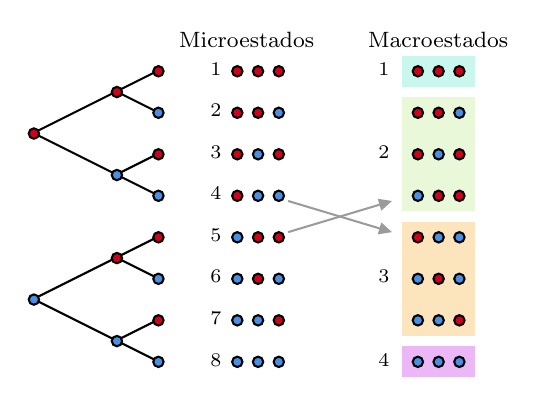
\begin{tikzpicture}[x=0.75pt,y=0.75pt,yscale=-1,xscale=1]
		%uncomment if require: \path (0,300); %set diagram left start at 0, and has height of 300
		
		%Straight Lines [id:da12481341037740112] 
		\draw    (47.25,57.25) -- (87.25,37.25) ;
		%Straight Lines [id:da3941446858209374] 
		\draw    (47.25,57.25) -- (87.25,77.25) ;
		%Straight Lines [id:da03529183420963489] 
		\draw    (87.25,37.25) -- (107.25,27.25) ;
		%Straight Lines [id:da3892371785701363] 
		\draw    (87.25,37.25) -- (107.25,47.25) ;
		%Straight Lines [id:da23333673411460487] 
		\draw    (87.25,77.25) -- (107.25,67.25) ;
		%Straight Lines [id:da7288749580642641] 
		\draw    (87.25,77.25) -- (107.25,87.25) ;
		%Straight Lines [id:da03471118792143546] 
		\draw    (47.25,137.25) -- (87.25,117.25) ;
		%Straight Lines [id:da8708899063640484] 
		\draw    (47.25,137.25) -- (87.25,157.25) ;
		%Straight Lines [id:da2899162244554536] 
		\draw    (87.25,117.25) -- (107.25,107.25) ;
		%Straight Lines [id:da39416608149949206] 
		\draw    (87.25,117.25) -- (107.25,127.25) ;
		%Straight Lines [id:da40862070962058006] 
		\draw    (87.25,157.25) -- (107.25,147.25) ;
		%Straight Lines [id:da2651254156316504] 
		\draw    (87.25,157.25) -- (107.25,167.25) ;
		%Shape: Circle [id:dp457665883774253] 
		\draw  [fill={rgb, 255:red, 208; green, 2; blue, 27 }  ,fill opacity=1 ] (45,57.5) .. controls (45,56.12) and (46.12,55) .. (47.5,55) .. controls (48.88,55) and (50,56.12) .. (50,57.5) .. controls (50,58.88) and (48.88,60) .. (47.5,60) .. controls (46.12,60) and (45,58.88) .. (45,57.5) -- cycle ;
		%Shape: Circle [id:dp9092299975589487] 
		\draw  [fill={rgb, 255:red, 208; green, 2; blue, 27 }  ,fill opacity=1 ] (85,37.5) .. controls (85,36.12) and (86.12,35) .. (87.5,35) .. controls (88.88,35) and (90,36.12) .. (90,37.5) .. controls (90,38.88) and (88.88,40) .. (87.5,40) .. controls (86.12,40) and (85,38.88) .. (85,37.5) -- cycle ;
		%Shape: Circle [id:dp44374044940504764] 
		\draw  [fill={rgb, 255:red, 208; green, 2; blue, 27 }  ,fill opacity=1 ] (105,27.5) .. controls (105,26.12) and (106.12,25) .. (107.5,25) .. controls (108.88,25) and (110,26.12) .. (110,27.5) .. controls (110,28.88) and (108.88,30) .. (107.5,30) .. controls (106.12,30) and (105,28.88) .. (105,27.5) -- cycle ;
		%Shape: Circle [id:dp2757721341329131] 
		\draw  [fill={rgb, 255:red, 208; green, 2; blue, 27 }  ,fill opacity=1 ] (105,67.5) .. controls (105,66.12) and (106.12,65) .. (107.5,65) .. controls (108.88,65) and (110,66.12) .. (110,67.5) .. controls (110,68.88) and (108.88,70) .. (107.5,70) .. controls (106.12,70) and (105,68.88) .. (105,67.5) -- cycle ;
		%Shape: Circle [id:dp8458867412596457] 
		\draw  [fill={rgb, 255:red, 208; green, 2; blue, 27 }  ,fill opacity=1 ] (85,117.5) .. controls (85,116.12) and (86.12,115) .. (87.5,115) .. controls (88.88,115) and (90,116.12) .. (90,117.5) .. controls (90,118.88) and (88.88,120) .. (87.5,120) .. controls (86.12,120) and (85,118.88) .. (85,117.5) -- cycle ;
		%Shape: Circle [id:dp676612446311422] 
		\draw  [fill={rgb, 255:red, 208; green, 2; blue, 27 }  ,fill opacity=1 ] (105,107.5) .. controls (105,106.12) and (106.12,105) .. (107.5,105) .. controls (108.88,105) and (110,106.12) .. (110,107.5) .. controls (110,108.88) and (108.88,110) .. (107.5,110) .. controls (106.12,110) and (105,108.88) .. (105,107.5) -- cycle ;
		%Shape: Circle [id:dp004383488974468719] 
		\draw  [fill={rgb, 255:red, 208; green, 2; blue, 27 }  ,fill opacity=1 ] (105,147.5) .. controls (105,146.12) and (106.12,145) .. (107.5,145) .. controls (108.88,145) and (110,146.12) .. (110,147.5) .. controls (110,148.88) and (108.88,150) .. (107.5,150) .. controls (106.12,150) and (105,148.88) .. (105,147.5) -- cycle ;
		%Shape: Circle [id:dp3171036714739712] 
		\draw  [fill={rgb, 255:red, 74; green, 144; blue, 226 }  ,fill opacity=1 ] (85,77.5) .. controls (85,76.12) and (86.12,75) .. (87.5,75) .. controls (88.88,75) and (90,76.12) .. (90,77.5) .. controls (90,78.88) and (88.88,80) .. (87.5,80) .. controls (86.12,80) and (85,78.88) .. (85,77.5) -- cycle ;
		%Shape: Circle [id:dp22555590641215484] 
		\draw  [fill={rgb, 255:red, 74; green, 144; blue, 226 }  ,fill opacity=1 ] (105,87.5) .. controls (105,86.12) and (106.12,85) .. (107.5,85) .. controls (108.88,85) and (110,86.12) .. (110,87.5) .. controls (110,88.88) and (108.88,90) .. (107.5,90) .. controls (106.12,90) and (105,88.88) .. (105,87.5) -- cycle ;
		%Shape: Circle [id:dp2925492736444313] 
		\draw  [fill={rgb, 255:red, 74; green, 144; blue, 226 }  ,fill opacity=1 ] (105,47.5) .. controls (105,46.12) and (106.12,45) .. (107.5,45) .. controls (108.88,45) and (110,46.12) .. (110,47.5) .. controls (110,48.88) and (108.88,50) .. (107.5,50) .. controls (106.12,50) and (105,48.88) .. (105,47.5) -- cycle ;
		%Shape: Circle [id:dp8406340157246389] 
		\draw  [fill={rgb, 255:red, 74; green, 144; blue, 226 }  ,fill opacity=1 ] (45,137.5) .. controls (45,136.12) and (46.12,135) .. (47.5,135) .. controls (48.88,135) and (50,136.12) .. (50,137.5) .. controls (50,138.88) and (48.88,140) .. (47.5,140) .. controls (46.12,140) and (45,138.88) .. (45,137.5) -- cycle ;
		%Shape: Circle [id:dp7966252914042035] 
		\draw  [fill={rgb, 255:red, 74; green, 144; blue, 226 }  ,fill opacity=1 ] (85,157.5) .. controls (85,156.12) and (86.12,155) .. (87.5,155) .. controls (88.88,155) and (90,156.12) .. (90,157.5) .. controls (90,158.88) and (88.88,160) .. (87.5,160) .. controls (86.12,160) and (85,158.88) .. (85,157.5) -- cycle ;
		%Shape: Circle [id:dp964732001141853] 
		\draw  [fill={rgb, 255:red, 74; green, 144; blue, 226 }  ,fill opacity=1 ] (105,167.5) .. controls (105,166.12) and (106.12,165) .. (107.5,165) .. controls (108.88,165) and (110,166.12) .. (110,167.5) .. controls (110,168.88) and (108.88,170) .. (107.5,170) .. controls (106.12,170) and (105,168.88) .. (105,167.5) -- cycle ;
		%Shape: Circle [id:dp5937131307662324] 
		\draw  [fill={rgb, 255:red, 74; green, 144; blue, 226 }  ,fill opacity=1 ] (105,127.5) .. controls (105,126.12) and (106.12,125) .. (107.5,125) .. controls (108.88,125) and (110,126.12) .. (110,127.5) .. controls (110,128.88) and (108.88,130) .. (107.5,130) .. controls (106.12,130) and (105,128.88) .. (105,127.5) -- cycle ;
		%Shape: Circle [id:dp5031507316729806] 
		\draw  [fill={rgb, 255:red, 208; green, 2; blue, 27 }  ,fill opacity=1 ] (143,27.5) .. controls (143,26.12) and (144.12,25) .. (145.5,25) .. controls (146.88,25) and (148,26.12) .. (148,27.5) .. controls (148,28.88) and (146.88,30) .. (145.5,30) .. controls (144.12,30) and (143,28.88) .. (143,27.5) -- cycle ;
		%Shape: Circle [id:dp4257463067614531] 
		\draw  [fill={rgb, 255:red, 208; green, 2; blue, 27 }  ,fill opacity=1 ] (153,27.5) .. controls (153,26.12) and (154.12,25) .. (155.5,25) .. controls (156.88,25) and (158,26.12) .. (158,27.5) .. controls (158,28.88) and (156.88,30) .. (155.5,30) .. controls (154.12,30) and (153,28.88) .. (153,27.5) -- cycle ;
		%Shape: Circle [id:dp25021307782417046] 
		\draw  [fill={rgb, 255:red, 208; green, 2; blue, 27 }  ,fill opacity=1 ] (163,27.5) .. controls (163,26.12) and (164.12,25) .. (165.5,25) .. controls (166.88,25) and (168,26.12) .. (168,27.5) .. controls (168,28.88) and (166.88,30) .. (165.5,30) .. controls (164.12,30) and (163,28.88) .. (163,27.5) -- cycle ;
		%Shape: Circle [id:dp16756063199628446] 
		\draw  [fill={rgb, 255:red, 208; green, 2; blue, 27 }  ,fill opacity=1 ] (143,47.5) .. controls (143,46.12) and (144.12,45) .. (145.5,45) .. controls (146.88,45) and (148,46.12) .. (148,47.5) .. controls (148,48.88) and (146.88,50) .. (145.5,50) .. controls (144.12,50) and (143,48.88) .. (143,47.5) -- cycle ;
		%Shape: Circle [id:dp5297292595701084] 
		\draw  [fill={rgb, 255:red, 208; green, 2; blue, 27 }  ,fill opacity=1 ] (153,47.5) .. controls (153,46.12) and (154.12,45) .. (155.5,45) .. controls (156.88,45) and (158,46.12) .. (158,47.5) .. controls (158,48.88) and (156.88,50) .. (155.5,50) .. controls (154.12,50) and (153,48.88) .. (153,47.5) -- cycle ;
		%Shape: Circle [id:dp4454918758783498] 
		\draw  [fill={rgb, 255:red, 208; green, 2; blue, 27 }  ,fill opacity=1 ] (143,67.5) .. controls (143,66.12) and (144.12,65) .. (145.5,65) .. controls (146.88,65) and (148,66.12) .. (148,67.5) .. controls (148,68.88) and (146.88,70) .. (145.5,70) .. controls (144.12,70) and (143,68.88) .. (143,67.5) -- cycle ;
		%Shape: Circle [id:dp23172188656161297] 
		\draw  [fill={rgb, 255:red, 208; green, 2; blue, 27 }  ,fill opacity=1 ] (143,87.5) .. controls (143,86.12) and (144.12,85) .. (145.5,85) .. controls (146.88,85) and (148,86.12) .. (148,87.5) .. controls (148,88.88) and (146.88,90) .. (145.5,90) .. controls (144.12,90) and (143,88.88) .. (143,87.5) -- cycle ;
		%Shape: Circle [id:dp9156123483432048] 
		\draw  [fill={rgb, 255:red, 208; green, 2; blue, 27 }  ,fill opacity=1 ] (163,67.5) .. controls (163,66.12) and (164.12,65) .. (165.5,65) .. controls (166.88,65) and (168,66.12) .. (168,67.5) .. controls (168,68.88) and (166.88,70) .. (165.5,70) .. controls (164.12,70) and (163,68.88) .. (163,67.5) -- cycle ;
		%Shape: Circle [id:dp6684401721083513] 
		\draw  [fill={rgb, 255:red, 208; green, 2; blue, 27 }  ,fill opacity=1 ] (153,107.5) .. controls (153,106.12) and (154.12,105) .. (155.5,105) .. controls (156.88,105) and (158,106.12) .. (158,107.5) .. controls (158,108.88) and (156.88,110) .. (155.5,110) .. controls (154.12,110) and (153,108.88) .. (153,107.5) -- cycle ;
		%Shape: Circle [id:dp9980139764740869] 
		\draw  [fill={rgb, 255:red, 208; green, 2; blue, 27 }  ,fill opacity=1 ] (163,107.5) .. controls (163,106.12) and (164.12,105) .. (165.5,105) .. controls (166.88,105) and (168,106.12) .. (168,107.5) .. controls (168,108.88) and (166.88,110) .. (165.5,110) .. controls (164.12,110) and (163,108.88) .. (163,107.5) -- cycle ;
		%Shape: Circle [id:dp7256376551180421] 
		\draw  [fill={rgb, 255:red, 208; green, 2; blue, 27 }  ,fill opacity=1 ] (163,147.5) .. controls (163,146.12) and (164.12,145) .. (165.5,145) .. controls (166.88,145) and (168,146.12) .. (168,147.5) .. controls (168,148.88) and (166.88,150) .. (165.5,150) .. controls (164.12,150) and (163,148.88) .. (163,147.5) -- cycle ;
		%Shape: Circle [id:dp7108108266443866] 
		\draw  [fill={rgb, 255:red, 74; green, 144; blue, 226 }  ,fill opacity=1 ] (163,47.5) .. controls (163,46.12) and (164.12,45) .. (165.5,45) .. controls (166.88,45) and (168,46.12) .. (168,47.5) .. controls (168,48.88) and (166.88,50) .. (165.5,50) .. controls (164.12,50) and (163,48.88) .. (163,47.5) -- cycle ;
		%Shape: Circle [id:dp08704503734337754] 
		\draw  [fill={rgb, 255:red, 74; green, 144; blue, 226 }  ,fill opacity=1 ] (153,67.5) .. controls (153,66.12) and (154.12,65) .. (155.5,65) .. controls (156.88,65) and (158,66.12) .. (158,67.5) .. controls (158,68.88) and (156.88,70) .. (155.5,70) .. controls (154.12,70) and (153,68.88) .. (153,67.5) -- cycle ;
		%Shape: Circle [id:dp4166577032002301] 
		\draw  [fill={rgb, 255:red, 74; green, 144; blue, 226 }  ,fill opacity=1 ] (153,87.5) .. controls (153,86.12) and (154.12,85) .. (155.5,85) .. controls (156.88,85) and (158,86.12) .. (158,87.5) .. controls (158,88.88) and (156.88,90) .. (155.5,90) .. controls (154.12,90) and (153,88.88) .. (153,87.5) -- cycle ;
		%Shape: Circle [id:dp8859075588551457] 
		\draw  [fill={rgb, 255:red, 74; green, 144; blue, 226 }  ,fill opacity=1 ] (163,87.5) .. controls (163,86.12) and (164.12,85) .. (165.5,85) .. controls (166.88,85) and (168,86.12) .. (168,87.5) .. controls (168,88.88) and (166.88,90) .. (165.5,90) .. controls (164.12,90) and (163,88.88) .. (163,87.5) -- cycle ;
		%Shape: Circle [id:dp1624674831412073] 
		\draw  [fill={rgb, 255:red, 74; green, 144; blue, 226 }  ,fill opacity=1 ] (143,107.5) .. controls (143,106.12) and (144.12,105) .. (145.5,105) .. controls (146.88,105) and (148,106.12) .. (148,107.5) .. controls (148,108.88) and (146.88,110) .. (145.5,110) .. controls (144.12,110) and (143,108.88) .. (143,107.5) -- cycle ;
		%Shape: Circle [id:dp880263714595793] 
		\draw  [fill={rgb, 255:red, 74; green, 144; blue, 226 }  ,fill opacity=1 ] (163,127.5) .. controls (163,126.12) and (164.12,125) .. (165.5,125) .. controls (166.88,125) and (168,126.12) .. (168,127.5) .. controls (168,128.88) and (166.88,130) .. (165.5,130) .. controls (164.12,130) and (163,128.88) .. (163,127.5) -- cycle ;
		%Shape: Circle [id:dp6223932023693238] 
		\draw  [fill={rgb, 255:red, 74; green, 144; blue, 226 }  ,fill opacity=1 ] (143,127.5) .. controls (143,126.12) and (144.12,125) .. (145.5,125) .. controls (146.88,125) and (148,126.12) .. (148,127.5) .. controls (148,128.88) and (146.88,130) .. (145.5,130) .. controls (144.12,130) and (143,128.88) .. (143,127.5) -- cycle ;
		%Shape: Circle [id:dp2234755928717046] 
		\draw  [fill={rgb, 255:red, 74; green, 144; blue, 226 }  ,fill opacity=1 ] (153,147.5) .. controls (153,146.12) and (154.12,145) .. (155.5,145) .. controls (156.88,145) and (158,146.12) .. (158,147.5) .. controls (158,148.88) and (156.88,150) .. (155.5,150) .. controls (154.12,150) and (153,148.88) .. (153,147.5) -- cycle ;
		%Shape: Circle [id:dp12439761199145549] 
		\draw  [fill={rgb, 255:red, 74; green, 144; blue, 226 }  ,fill opacity=1 ] (143,147.5) .. controls (143,146.12) and (144.12,145) .. (145.5,145) .. controls (146.88,145) and (148,146.12) .. (148,147.5) .. controls (148,148.88) and (146.88,150) .. (145.5,150) .. controls (144.12,150) and (143,148.88) .. (143,147.5) -- cycle ;
		%Shape: Circle [id:dp07500475785680516] 
		\draw  [fill={rgb, 255:red, 74; green, 144; blue, 226 }  ,fill opacity=1 ] (143,167.5) .. controls (143,166.12) and (144.12,165) .. (145.5,165) .. controls (146.88,165) and (148,166.12) .. (148,167.5) .. controls (148,168.88) and (146.88,170) .. (145.5,170) .. controls (144.12,170) and (143,168.88) .. (143,167.5) -- cycle ;
		%Shape: Circle [id:dp4516586097257167] 
		\draw  [fill={rgb, 255:red, 74; green, 144; blue, 226 }  ,fill opacity=1 ] (153,167.5) .. controls (153,166.12) and (154.12,165) .. (155.5,165) .. controls (156.88,165) and (158,166.12) .. (158,167.5) .. controls (158,168.88) and (156.88,170) .. (155.5,170) .. controls (154.12,170) and (153,168.88) .. (153,167.5) -- cycle ;
		%Shape: Circle [id:dp18892437450888744] 
		\draw  [fill={rgb, 255:red, 74; green, 144; blue, 226 }  ,fill opacity=1 ] (163,167.5) .. controls (163,166.12) and (164.12,165) .. (165.5,165) .. controls (166.88,165) and (168,166.12) .. (168,167.5) .. controls (168,168.88) and (166.88,170) .. (165.5,170) .. controls (164.12,170) and (163,168.88) .. (163,167.5) -- cycle ;
		%Shape: Circle [id:dp21734893282637857] 
		\draw  [fill={rgb, 255:red, 208; green, 2; blue, 27 }  ,fill opacity=1 ] (153,127.5) .. controls (153,126.12) and (154.12,125) .. (155.5,125) .. controls (156.88,125) and (158,126.12) .. (158,127.5) .. controls (158,128.88) and (156.88,130) .. (155.5,130) .. controls (154.12,130) and (153,128.88) .. (153,127.5) -- cycle ;
		%Shape: Rectangle [id:dp5826645305943808] 
		\draw  [draw opacity=0][fill={rgb, 255:red, 245; green, 166; blue, 35 }  ,fill opacity=0.3 ] (225,100) -- (260,100) -- (260,155) -- (225,155) -- cycle ;
		%Shape: Rectangle [id:dp08785252833573987] 
		\draw  [draw opacity=0][fill={rgb, 255:red, 189; green, 16; blue, 224 }  ,fill opacity=0.3 ] (225,160) -- (260,160) -- (260,175) -- (225,175) -- cycle ;
		%Shape: Rectangle [id:dp3413459650451903] 
		\draw  [draw opacity=0][fill={rgb, 255:red, 184; green, 233; blue, 134 }  ,fill opacity=0.3 ] (225,40) -- (260,40) -- (260,95) -- (225,95) -- cycle ;
		%Shape: Rectangle [id:dp7604234047032441] 
		\draw  [draw opacity=0][fill={rgb, 255:red, 80; green, 227; blue, 194 }  ,fill opacity=0.3 ] (225,20) -- (260,20) -- (260,35) -- (225,35) -- cycle ;
		%Shape: Circle [id:dp8973199509716385] 
		\draw  [fill={rgb, 255:red, 208; green, 2; blue, 27 }  ,fill opacity=1 ] (230,27.5) .. controls (230,26.12) and (231.12,25) .. (232.5,25) .. controls (233.88,25) and (235,26.12) .. (235,27.5) .. controls (235,28.88) and (233.88,30) .. (232.5,30) .. controls (231.12,30) and (230,28.88) .. (230,27.5) -- cycle ;
		%Shape: Circle [id:dp4575477256963427] 
		\draw  [fill={rgb, 255:red, 208; green, 2; blue, 27 }  ,fill opacity=1 ] (240,27.5) .. controls (240,26.12) and (241.12,25) .. (242.5,25) .. controls (243.88,25) and (245,26.12) .. (245,27.5) .. controls (245,28.88) and (243.88,30) .. (242.5,30) .. controls (241.12,30) and (240,28.88) .. (240,27.5) -- cycle ;
		%Shape: Circle [id:dp23625244340802065] 
		\draw  [fill={rgb, 255:red, 208; green, 2; blue, 27 }  ,fill opacity=1 ] (250,27.5) .. controls (250,26.12) and (251.12,25) .. (252.5,25) .. controls (253.88,25) and (255,26.12) .. (255,27.5) .. controls (255,28.88) and (253.88,30) .. (252.5,30) .. controls (251.12,30) and (250,28.88) .. (250,27.5) -- cycle ;
		%Shape: Circle [id:dp29254579159186145] 
		\draw  [fill={rgb, 255:red, 208; green, 2; blue, 27 }  ,fill opacity=1 ] (230,47.5) .. controls (230,46.12) and (231.12,45) .. (232.5,45) .. controls (233.88,45) and (235,46.12) .. (235,47.5) .. controls (235,48.88) and (233.88,50) .. (232.5,50) .. controls (231.12,50) and (230,48.88) .. (230,47.5) -- cycle ;
		%Shape: Circle [id:dp41477766508813074] 
		\draw  [fill={rgb, 255:red, 208; green, 2; blue, 27 }  ,fill opacity=1 ] (240,47.5) .. controls (240,46.12) and (241.12,45) .. (242.5,45) .. controls (243.88,45) and (245,46.12) .. (245,47.5) .. controls (245,48.88) and (243.88,50) .. (242.5,50) .. controls (241.12,50) and (240,48.88) .. (240,47.5) -- cycle ;
		%Shape: Circle [id:dp22857637209155457] 
		\draw  [fill={rgb, 255:red, 208; green, 2; blue, 27 }  ,fill opacity=1 ] (230,67.5) .. controls (230,66.12) and (231.12,65) .. (232.5,65) .. controls (233.88,65) and (235,66.12) .. (235,67.5) .. controls (235,68.88) and (233.88,70) .. (232.5,70) .. controls (231.12,70) and (230,68.88) .. (230,67.5) -- cycle ;
		%Shape: Circle [id:dp5902864724303766] 
		\draw  [fill={rgb, 255:red, 208; green, 2; blue, 27 }  ,fill opacity=1 ] (230,107.5) .. controls (230,106.12) and (231.12,105) .. (232.5,105) .. controls (233.88,105) and (235,106.12) .. (235,107.5) .. controls (235,108.88) and (233.88,110) .. (232.5,110) .. controls (231.12,110) and (230,108.88) .. (230,107.5) -- cycle ;
		%Shape: Circle [id:dp7581285806487291] 
		\draw  [fill={rgb, 255:red, 208; green, 2; blue, 27 }  ,fill opacity=1 ] (250,67.5) .. controls (250,66.12) and (251.12,65) .. (252.5,65) .. controls (253.88,65) and (255,66.12) .. (255,67.5) .. controls (255,68.88) and (253.88,70) .. (252.5,70) .. controls (251.12,70) and (250,68.88) .. (250,67.5) -- cycle ;
		%Shape: Circle [id:dp3507058156361318] 
		\draw  [fill={rgb, 255:red, 208; green, 2; blue, 27 }  ,fill opacity=1 ] (240,87.5) .. controls (240,86.12) and (241.12,85) .. (242.5,85) .. controls (243.88,85) and (245,86.12) .. (245,87.5) .. controls (245,88.88) and (243.88,90) .. (242.5,90) .. controls (241.12,90) and (240,88.88) .. (240,87.5) -- cycle ;
		%Shape: Circle [id:dp11646210505307808] 
		\draw  [fill={rgb, 255:red, 208; green, 2; blue, 27 }  ,fill opacity=1 ] (250,87.5) .. controls (250,86.12) and (251.12,85) .. (252.5,85) .. controls (253.88,85) and (255,86.12) .. (255,87.5) .. controls (255,88.88) and (253.88,90) .. (252.5,90) .. controls (251.12,90) and (250,88.88) .. (250,87.5) -- cycle ;
		%Shape: Circle [id:dp3774230818097182] 
		\draw  [fill={rgb, 255:red, 208; green, 2; blue, 27 }  ,fill opacity=1 ] (250,147.5) .. controls (250,146.12) and (251.12,145) .. (252.5,145) .. controls (253.88,145) and (255,146.12) .. (255,147.5) .. controls (255,148.88) and (253.88,150) .. (252.5,150) .. controls (251.12,150) and (250,148.88) .. (250,147.5) -- cycle ;
		%Shape: Circle [id:dp08285638517594307] 
		\draw  [fill={rgb, 255:red, 74; green, 144; blue, 226 }  ,fill opacity=1 ] (250,47.5) .. controls (250,46.12) and (251.12,45) .. (252.5,45) .. controls (253.88,45) and (255,46.12) .. (255,47.5) .. controls (255,48.88) and (253.88,50) .. (252.5,50) .. controls (251.12,50) and (250,48.88) .. (250,47.5) -- cycle ;
		%Shape: Circle [id:dp49581810992593633] 
		\draw  [fill={rgb, 255:red, 74; green, 144; blue, 226 }  ,fill opacity=1 ] (240,67.5) .. controls (240,66.12) and (241.12,65) .. (242.5,65) .. controls (243.88,65) and (245,66.12) .. (245,67.5) .. controls (245,68.88) and (243.88,70) .. (242.5,70) .. controls (241.12,70) and (240,68.88) .. (240,67.5) -- cycle ;
		%Shape: Circle [id:dp6428138923677286] 
		\draw  [fill={rgb, 255:red, 74; green, 144; blue, 226 }  ,fill opacity=1 ] (240,107.5) .. controls (240,106.12) and (241.12,105) .. (242.5,105) .. controls (243.88,105) and (245,106.12) .. (245,107.5) .. controls (245,108.88) and (243.88,110) .. (242.5,110) .. controls (241.12,110) and (240,108.88) .. (240,107.5) -- cycle ;
		%Shape: Circle [id:dp7905037923710481] 
		\draw  [fill={rgb, 255:red, 74; green, 144; blue, 226 }  ,fill opacity=1 ] (250,107.5) .. controls (250,106.12) and (251.12,105) .. (252.5,105) .. controls (253.88,105) and (255,106.12) .. (255,107.5) .. controls (255,108.88) and (253.88,110) .. (252.5,110) .. controls (251.12,110) and (250,108.88) .. (250,107.5) -- cycle ;
		%Shape: Circle [id:dp48039181267926023] 
		\draw  [fill={rgb, 255:red, 74; green, 144; blue, 226 }  ,fill opacity=1 ] (230,87.5) .. controls (230,86.12) and (231.12,85) .. (232.5,85) .. controls (233.88,85) and (235,86.12) .. (235,87.5) .. controls (235,88.88) and (233.88,90) .. (232.5,90) .. controls (231.12,90) and (230,88.88) .. (230,87.5) -- cycle ;
		%Shape: Circle [id:dp24843359292740996] 
		\draw  [fill={rgb, 255:red, 74; green, 144; blue, 226 }  ,fill opacity=1 ] (250,127.5) .. controls (250,126.12) and (251.12,125) .. (252.5,125) .. controls (253.88,125) and (255,126.12) .. (255,127.5) .. controls (255,128.88) and (253.88,130) .. (252.5,130) .. controls (251.12,130) and (250,128.88) .. (250,127.5) -- cycle ;
		%Shape: Circle [id:dp1497368885199094] 
		\draw  [fill={rgb, 255:red, 74; green, 144; blue, 226 }  ,fill opacity=1 ] (230,127.5) .. controls (230,126.12) and (231.12,125) .. (232.5,125) .. controls (233.88,125) and (235,126.12) .. (235,127.5) .. controls (235,128.88) and (233.88,130) .. (232.5,130) .. controls (231.12,130) and (230,128.88) .. (230,127.5) -- cycle ;
		%Shape: Circle [id:dp9266830734895113] 
		\draw  [fill={rgb, 255:red, 74; green, 144; blue, 226 }  ,fill opacity=1 ] (240,147.5) .. controls (240,146.12) and (241.12,145) .. (242.5,145) .. controls (243.88,145) and (245,146.12) .. (245,147.5) .. controls (245,148.88) and (243.88,150) .. (242.5,150) .. controls (241.12,150) and (240,148.88) .. (240,147.5) -- cycle ;
		%Shape: Circle [id:dp58477948816646] 
		\draw  [fill={rgb, 255:red, 74; green, 144; blue, 226 }  ,fill opacity=1 ] (230,147.5) .. controls (230,146.12) and (231.12,145) .. (232.5,145) .. controls (233.88,145) and (235,146.12) .. (235,147.5) .. controls (235,148.88) and (233.88,150) .. (232.5,150) .. controls (231.12,150) and (230,148.88) .. (230,147.5) -- cycle ;
		%Shape: Circle [id:dp668743602338472] 
		\draw  [fill={rgb, 255:red, 74; green, 144; blue, 226 }  ,fill opacity=1 ] (230,167.5) .. controls (230,166.12) and (231.12,165) .. (232.5,165) .. controls (233.88,165) and (235,166.12) .. (235,167.5) .. controls (235,168.88) and (233.88,170) .. (232.5,170) .. controls (231.12,170) and (230,168.88) .. (230,167.5) -- cycle ;
		%Shape: Circle [id:dp7201517341198097] 
		\draw  [fill={rgb, 255:red, 74; green, 144; blue, 226 }  ,fill opacity=1 ] (240,167.5) .. controls (240,166.12) and (241.12,165) .. (242.5,165) .. controls (243.88,165) and (245,166.12) .. (245,167.5) .. controls (245,168.88) and (243.88,170) .. (242.5,170) .. controls (241.12,170) and (240,168.88) .. (240,167.5) -- cycle ;
		%Shape: Circle [id:dp6799103083398305] 
		\draw  [fill={rgb, 255:red, 74; green, 144; blue, 226 }  ,fill opacity=1 ] (250,167.5) .. controls (250,166.12) and (251.12,165) .. (252.5,165) .. controls (253.88,165) and (255,166.12) .. (255,167.5) .. controls (255,168.88) and (253.88,170) .. (252.5,170) .. controls (251.12,170) and (250,168.88) .. (250,167.5) -- cycle ;
		%Shape: Circle [id:dp487759295058546] 
		\draw  [fill={rgb, 255:red, 208; green, 2; blue, 27 }  ,fill opacity=1 ] (240,127.5) .. controls (240,126.12) and (241.12,125) .. (242.5,125) .. controls (243.88,125) and (245,126.12) .. (245,127.5) .. controls (245,128.88) and (243.88,130) .. (242.5,130) .. controls (241.12,130) and (240,128.88) .. (240,127.5) -- cycle ;
		%Straight Lines [id:da8843808827658718] 
		\draw [color={rgb, 255:red, 155; green, 155; blue, 155 }  ,draw opacity=1 ]   (170,90) -- (217.13,104.14) ;
		\draw [shift={(220,105)}, rotate = 196.7] [fill={rgb, 255:red, 155; green, 155; blue, 155 }  ,fill opacity=1 ][line width=0.08]  [draw opacity=0] (6.25,-3) -- (0,0) -- (6.25,3) -- cycle    ;
		%Straight Lines [id:da18531733349774127] 
		\draw [color={rgb, 255:red, 155; green, 155; blue, 155 }  ,draw opacity=1 ]   (170,105) -- (217.13,90.86) ;
		\draw [shift={(220,90)}, rotate = 163.3] [fill={rgb, 255:red, 155; green, 155; blue, 155 }  ,fill opacity=1 ][line width=0.08]  [draw opacity=0] (6.25,-3) -- (0,0) -- (6.25,3) -- cycle    ;
		
		% Text Node
		\draw (116,7) node [anchor=north west][inner sep=0.75pt]  [font=\footnotesize] [align=left] {Microestados};
		% Text Node
		\draw (207,7) node [anchor=north west][inner sep=0.75pt]  [font=\footnotesize] [align=left] {Macroestados};
		% Text Node
		\draw (131,22) node [anchor=north west][inner sep=0.75pt]  [font=\scriptsize] [align=left] {1};
		% Text Node
		\draw (131,42) node [anchor=north west][inner sep=0.75pt]  [font=\scriptsize] [align=left] {2};
		% Text Node
		\draw (131,62) node [anchor=north west][inner sep=0.75pt]  [font=\scriptsize] [align=left] {3};
		% Text Node
		\draw (131,82) node [anchor=north west][inner sep=0.75pt]  [font=\scriptsize] [align=left] {4};
		% Text Node
		\draw (131,102) node [anchor=north west][inner sep=0.75pt]  [font=\scriptsize] [align=left] {5};
		% Text Node
		\draw (131,122) node [anchor=north west][inner sep=0.75pt]  [font=\scriptsize] [align=left] {6};
		% Text Node
		\draw (131,142) node [anchor=north west][inner sep=0.75pt]  [font=\scriptsize] [align=left] {7};
		% Text Node
		\draw (131,162) node [anchor=north west][inner sep=0.75pt]  [font=\scriptsize] [align=left] {8};
		% Text Node
		\draw (212,22) node [anchor=north west][inner sep=0.75pt]  [font=\scriptsize] [align=left] {1};
		% Text Node
		\draw (212,62) node [anchor=north west][inner sep=0.75pt]  [font=\scriptsize] [align=left] {2};
		% Text Node
		\draw (212,122) node [anchor=north west][inner sep=0.75pt]  [font=\scriptsize] [align=left] {3};
		% Text Node
		\draw (212,162) node [anchor=north west][inner sep=0.75pt]  [font=\scriptsize] [align=left] {4};	
	\end{tikzpicture}
\end{figure}

\caja{Microestado}{Cada arreglo particular posible en los que puede	encontrarse el sistema estudiado.}
\caja{Macroestado}{El conjunto de microestados iguales.}
\subsection{Postulados fundamentales}
\begin{enumerate}
	\item \textbf{Primer postulado:} La probabilidad de obtener cualquier microestado es la misma para todos los microestados en un sistema en equilibrio.
	\item \textbf{Segundo postulado:} El macroestado más probable es el que tenga el mayor número de
	microestados para un sistema en	equilibrio.
\end{enumerate}
Para un sistema clásico de \(N\) partículas tendremos un espacio de fase \(\Gamma\) (es decir, un conjunto de variables independientes) formado por las posiciones y momentos posibles de cada partícula:
\begin{equation}
	\Gamma = (q_1,\ldots,q_N,p_1,\ldots,p_N) \in \mathbb{R}^{6N}
\end{equation}
y la dinámica está gobernada por un Hamiltoniano \(H(\Gamma)\).

Para construir el elemento volumétrico infinitesimal partimos de la noción clásica de:
\begin{equation*}
	d^{3N}q d^{3N}p = dq_1 \ldots dq_N dp_1 \ldots dp_N
\end{equation*}
con dos correcciones: un factor \(1/N!\), para considerar la indistinguibilidad de las partículas idénticas; y otro factor \(1/h^{3N}\), para cuantizar las celdas más pequeñas del espacio. Tendremos entonces:
\begin{equation}
	d\Gamma = \frac{1}{N!h^{3N}}d^{3N}q d^{3N}p
\end{equation}
donde \(h\) es la constante de Planck.

Considerando la densidad de probabilidad \(\rho(\Gamma, t)\) en el espacio de fases, el teorema de Liouville nos dice que la probabilidad en un volumen debe conservarse, por lo que considerando una ecuación de continuidad:
\begin{equation}
	\frac{d\rho}{dt} = 0
\end{equation}
En equilibrio, \(\rho\) no depende explícitamente del tiempo. Por lo tanto, los ensambles de equilibrio (microcanónico, canónico, gran canónico) se construyen como distribuciones que son funciones de las constantes de movimiento, siendo la más común la energía.
\begin{figure}[h]
	\centering
	% Gradient Info
	
	\tikzset {_rd6rtips6/.code = {\pgfsetadditionalshadetransform{ \pgftransformshift{\pgfpoint{97.2 bp } { -118.8 bp }  }  \pgftransformscale{1.44 }  }}}
	\pgfdeclareradialshading{_k1ybqqjt0}{\pgfpoint{-72bp}{88bp}}{rgb(0bp)=(0.29,0.56,0.89);
		rgb(0bp)=(0.29,0.56,0.89);
		rgb(25bp)=(0.93,0.33,0.41);
		rgb(400bp)=(0.93,0.33,0.41)}
	
	% Gradient Info
	
	\tikzset {_2ap19e4iz/.code = {\pgfsetadditionalshadetransform{ \pgftransformshift{\pgfpoint{0 bp } { 0 bp }  }  \pgftransformrotate{-90 }  \pgftransformscale{2 }  }}}
	\pgfdeclarehorizontalshading{_92siszo40}{150bp}{rgb(0bp)=(0.29,0.56,0.89);
		rgb(37.5bp)=(0.29,0.56,0.89);
		rgb(62.5bp)=(0.93,0.33,0.41);
		rgb(100bp)=(0.93,0.33,0.41)}
	
	% Gradient Info
	
	\tikzset {_pom7hki1c/.code = {\pgfsetadditionalshadetransform{ \pgftransformshift{\pgfpoint{97.2 bp } { -118.8 bp }  }  \pgftransformscale{1.44 }  }}}
	\pgfdeclareradialshading{_8tqegm4rf}{\pgfpoint{-72bp}{88bp}}{rgb(0bp)=(0.29,0.56,0.89);
		rgb(0bp)=(0.29,0.56,0.89);
		rgb(25bp)=(0.93,0.33,0.41);
		rgb(400bp)=(0.93,0.33,0.41)}
	
	% Gradient Info
	
	\tikzset {_w8zz6jh42/.code = {\pgfsetadditionalshadetransform{ \pgftransformshift{\pgfpoint{0 bp } { 0 bp }  }  \pgftransformrotate{-90 }  \pgftransformscale{2 }  }}}
	\pgfdeclarehorizontalshading{_8tfhuszfr}{150bp}{rgb(0bp)=(0.29,0.56,0.89);
		rgb(37.5bp)=(0.29,0.56,0.89);
		rgb(62.5bp)=(0.93,0.33,0.41);
		rgb(100bp)=(0.93,0.33,0.41)}
	\tikzset{every picture/.style={line width=0.75pt}} %set default line width to 0.75pt        
	
	\begin{tikzpicture}[x=0.75pt,y=0.75pt,yscale=-1,xscale=1]
		%uncomment if require: \path (0,300); %set diagram left start at 0, and has height of 300
		
		%Shape: Axis 2D [id:dp11941702079298011] 
		\draw  (10,155) -- (160,155)(25,20) -- (25,170) (153,150) -- (160,155) -- (153,160) (20,27) -- (25,20) -- (30,27)  ;
		%Flowchart: Punched Tape [id:dp29547391851155225] 
		\path  [shading=_k1ybqqjt0,_rd6rtips6] (45,61) .. controls (45,64.31) and (52.28,67) .. (61.25,67) .. controls (70.22,67) and (77.5,64.31) .. (77.5,61) .. controls (77.5,57.69) and (84.78,55) .. (93.75,55) .. controls (102.72,55) and (110,57.69) .. (110,61) -- (110,109) .. controls (110,105.69) and (102.72,103) .. (93.75,103) .. controls (84.78,103) and (77.5,105.69) .. (77.5,109) .. controls (77.5,112.31) and (70.22,115) .. (61.25,115) .. controls (52.28,115) and (45,112.31) .. (45,109) -- cycle ; % for fading 
		\draw   (45,61) .. controls (45,64.31) and (52.28,67) .. (61.25,67) .. controls (70.22,67) and (77.5,64.31) .. (77.5,61) .. controls (77.5,57.69) and (84.78,55) .. (93.75,55) .. controls (102.72,55) and (110,57.69) .. (110,61) -- (110,109) .. controls (110,105.69) and (102.72,103) .. (93.75,103) .. controls (84.78,103) and (77.5,105.69) .. (77.5,109) .. controls (77.5,112.31) and (70.22,115) .. (61.25,115) .. controls (52.28,115) and (45,112.31) .. (45,109) -- cycle ; % for border 
		
		%Shape: Rectangle [id:dp24490765244567625] 
		\path  [shading=_92siszo40,_2ap19e4iz] (140,40) -- (150,40) -- (150,140) -- (140,140) -- cycle ; % for fading 
		\draw  [line width=0.75]  (140,40) -- (150,40) -- (150,140) -- (140,140) -- cycle ; % for border 
		
		%Shape: Axis 2D [id:dp5614637097431934] 
		\draw  (215,155) -- (365,155)(230,20) -- (230,170) (358,150) -- (365,155) -- (358,160) (225,27) -- (230,20) -- (235,27)  ;
		%Flowchart: Punched Tape [id:dp8054452460561271] 
		\path  [shading=_8tqegm4rf,_pom7hki1c] (275,32) .. controls (275,38.63) and (277.24,44) .. (280,44) .. controls (282.76,44) and (285,38.63) .. (285,32) .. controls (285,25.37) and (287.24,20) .. (290,20) .. controls (292.76,20) and (295,25.37) .. (295,32) -- (295,128) .. controls (295,121.37) and (292.76,116) .. (290,116) .. controls (287.24,116) and (285,121.37) .. (285,128) .. controls (285,134.63) and (282.76,140) .. (280,140) .. controls (277.24,140) and (275,134.63) .. (275,128) -- cycle ; % for fading 
		\draw   (275,32) .. controls (275,38.63) and (277.24,44) .. (280,44) .. controls (282.76,44) and (285,38.63) .. (285,32) .. controls (285,25.37) and (287.24,20) .. (290,20) .. controls (292.76,20) and (295,25.37) .. (295,32) -- (295,128) .. controls (295,121.37) and (292.76,116) .. (290,116) .. controls (287.24,116) and (285,121.37) .. (285,128) .. controls (285,134.63) and (282.76,140) .. (280,140) .. controls (277.24,140) and (275,134.63) .. (275,128) -- cycle ; % for border 
		
		%Shape: Rectangle [id:dp1530763046716347] 
		\path  [shading=_8tfhuszfr,_w8zz6jh42] (345,40) -- (355,40) -- (355,140) -- (345,140) -- cycle ; % for fading 
		\draw  [line width=0.75]  (345,40) -- (355,40) -- (355,140) -- (345,140) -- cycle ; % for border 
		
		%Right Arrow [id:dp1977517253661314] 
		\draw   (165,85) -- (195,85) -- (195,80) -- (215,90) -- (195,100) -- (195,95) -- (165,95) -- cycle ;
		
		% Text Node
		\draw (181,67) node [anchor=north west][inner sep=0.75pt]   [align=left] {$\displaystyle t$};
		% Text Node
		\draw (126,20) node [anchor=north west][inner sep=0.75pt]   [align=left] {$\displaystyle \rho ( p,q)$};
		% Text Node
		\draw (331,20) node [anchor=north west][inner sep=0.75pt]   [align=left] {$\displaystyle \rho ( p,q)$};
		% Text Node
		\draw (156,160) node [anchor=north west][inner sep=0.75pt]   [align=left] {$\displaystyle p$};
		% Text Node
		\draw (361,160) node [anchor=north west][inner sep=0.75pt]   [align=left] {$\displaystyle p$};
		% Text Node
		\draw (8,15) node [anchor=north west][inner sep=0.75pt]   [align=left] {$\displaystyle q$};
		% Text Node
		\draw (213,17) node [anchor=north west][inner sep=0.75pt]   [align=left] {$\displaystyle q$};
		% Text Node
		\draw (56,120) node [anchor=north west][inner sep=0.75pt]   [align=left] {$\displaystyle V=V_{0}$};
		% Text Node
		\draw (263,140) node [anchor=north west][inner sep=0.75pt]   [align=left] {$\displaystyle V=V_{0}$};
	\end{tikzpicture}
\end{figure}

La conservación del volumen implica que la evolución es reversible y que la información sobre el estado inicial no se pierde (aunque en la práctica se vuelva inaccesible).

\subsubsection{Hipótesis Ergódica}
\caja{Ensamble}{Un conjunto o ensamble estadístico es una colección de un número muy grande de réplicas del sistema bajo estudio.}

El promedio temporal de una trayectoria única:
\begin{equation*}
	\bar{A} = \lim_{\tau\rightarrow\infty}\frac{1}{\tau}\int_{0}^{\tau}A(\Gamma(t))dt
\end{equation*}
y el promedio sobre un ensamble de sistemas con un volumen \(d\Gamma\):
\begin{equation*}
	\left\langle A\right\rangle = \int A(\Gamma)\rho(\Gamma)d\Gamma
\end{equation*}
La \textbf{hipótesis ergódica} consiste en postular que ambos promedios son equivalentes:
\begin{equation}
	\bar{A} = \left\langle A\right\rangle
\end{equation}
Para un tiempo lo suficientemente largo, cualquiera de los sistemas del conjunto contendrá todos los microestados posibles, con la particularidad que su tiempo relativo de permanencia en cada uno de los microestados es igual al número relativo de sistemas del conjunto que se encuentren en este microestado.

\subsection{Ensamble microcanónico}
\subsubsection{Postulado fundamental de Gibbs}
\caja{\textbf{Postulado de igual probabilidad a priori}}[blue!40][blue!20]{Para un sistema aislado en equilibrio, todos los microestados accesibles compatibles con \(E,V,N\) son equiprobables.}

Si tomamos el ejemplo de lanzar una moneda 3 veces y registrar su lado, obtendremos el conjunto de resultados \(\left\lbrace ccc, ccs, csc, css, scc, scs, ssc, sss \right\rbrace \). Asumiendo que todos estos microestados corresponden a un mismo nivel de energía, el postulado nos dice que no hay preferencia por ninguno de ellos.

Si la región accesible está restringida por
\begin{equation*}
	E \leq H(\Gamma) \leq E + \delta E ,
\end{equation*}
entonces
\begin{equation*}
	\rho_{\text{MC}}(\Gamma) = \frac{1}{\Omega(E,\delta E,V,N)}
\end{equation*}
en la capa de energía, y cero fuera de ella.

\subsubsection{Ensamble microcanónico}
Un conjunto estadístico de sistemas aislados se denomina \textbf{ensamble microcanónico}. Es decir, sistemas que mantienen \(E,V,N\) fijos.

En el ensamble microcanónico, \(\Omega(E,V,N)\) representa la \textbf{densidad de estados}:
\begin{equation}
	\Omega(E,V,N) = \frac{1}{N!h^{3N}}\int\delta(E-H(\Gamma))d\Gamma
\end{equation}
es decir, el número de microestados por unidad de energía alrededor de \(E\). También puede interpretarse (salvo constantes) como el área de la superficie de energía constante en el espacio de fases.

Además de la densidad de estados \(\Omega\), se define el \textbf{volumen acumulado}:
\begin{equation}
	\Phi(E,V,N) = \frac{1}{N!h^{3N}}\int_{H(\Gamma)\leq E}d\Gamma
\end{equation}
es decir, el volumen del espacio de fases con energía \(\leq E\). Ambas cantidades se relacionan mediante:
\begin{equation}
	\Omega(E,V,N) = \frac{\partial\Phi}{\partial E}
\end{equation}

\subsubsection{Entropía microcanónica}
En el ensamble microcanónico, la termodinámica emerge directamente de la geometría del espacio de fases accesible. A mayor volumen \(\Omega\), mayor entropía \(S\).

La entropía se define mediante la \textbf{relación de Boltzmann}:
\begin{equation}
	S(E,V,N) = k_B \ln{\Omega(E,V,N)}
\end{equation}
o su equivalente con \(\Phi\), que da la misma termodinámica en el límite termodinámico.

\subsubsection{Equilibrio térmico entre dos sistemas}
El equilibrio térmico entre dos sistemas se alcanza cuando sus temperaturas son iguales. La temperatura es el parámetro que se iguala al maximizar el número total de microestados.

Consideremos dos sistemas aislados \(A_1\) y \(A_2\), en equilibrio por separado:
\begin{itemize}
	\item \(\mathbf{A_1}\): \(N_1, V_1, E_1, \Omega_1(E_1,V_1,N_1)\)
	\item \(\mathbf{A_2}\): \(N_2, V_2, E_2, \Omega_2(E_2,V_2,N_2)\)
\end{itemize}
Al ponerlos en contacto térmico intercambian energía, pero no volumen ni partículas, formarán un sistema compuesto por:
\begin{equation*}
	E_1 + E_2 = E_0 \text{cte.}, N_1,N_2,V_1,V_2 \text{fijos}
\end{equation*}
El número total de microestados accesibles al sistema compuesto será:
\begin{equation}
	\Omega_0(E_1) = \Omega_1(E_1,V_1,N_1)\cdot\Omega_2(E_0-E_1,V_2,N_2)
\end{equation}
\textbf{Condición de equilibrio}: La energía se redistribuirá hasta maximizar \(\Omega_0(E_1)\):
\begin{equation}
	\left. \frac{\partial}{\partial E_1}\Omega_0(E_1)\right|_{E_1 = E_1^{\text{eq}}} = 0
\end{equation}
Luego, tomando logaritmos, derivando y utilizando la definición de temperatura, llegamos a que la condición de equilibrio es:
\begin{equation}
	T_1  = T_2
\end{equation}

\subsubsection{Equilibrio mecánico entre dos sistemas}
El equilibrio mecánico entre dos sistemas se alcanza cuando sus presiones son iguales.

Si ahora consideramos dos sistemas en contacto térmico (no aislados, a misma temperatura), pero separados por un pistón móvil que permite intercambiar volumen manteniendo igual el número de partículas:
\begin{itemize}
	\item \(\mathbf{A_1}\): \(N_1, V_1, T, \Omega_1(N_1,V_1,T)\)
	\item \(\mathbf{A_2}\): \(N_2, V_2, T, \Omega_2(N_2,V_2,T)\)
	\item Volumen constante: \(V_1 + V_2 = V_0\)
	\item \(N_1, N_2\) fijos
\end{itemize}
El número total de microestados accesibles al sistema compuesto será:
\begin{equation*}
	\Omega_0(V_1) = \Omega_1(N_1,V_1,T)\cdot\Omega_2(N_2,V_0-V_1,T)
\end{equation*}
La condición de equilibrio:
\begin{equation*}
	\left. \frac{\partial}{\partial V_1}\ln{\Omega_0}\right|_{V_1 = V_1^{\text{eq}}} = 0
\end{equation*}
Derivando:
\begin{equation}
	p_1 = p_2
\end{equation}

\subsubsection{Equilibrio químico entre dos sistemas}
El equilibrio químico entre dos sistemas se alcanza cuando sus potenciales químicos son iguales.

Si ahora consideramos dos sistemas en contacto térmico (no aislados, a misma temperatura), pero separados por una pared porosa que permite intercambiar partículas manteniendo igual el número de volumen:
\begin{itemize}
	\item \(\mathbf{A_1}\): \(N_1, V_1, T, \Omega_1(N_1,V_1,T)\)
	\item \(\mathbf{A_2}\): \(N_2, V_2, T, \Omega_2(N_2,V_2,T)\)
	\item Número total de partículas constante: \(N_1 + N_2 = N_0\)
	\item \(V_1, V_2\) fijos
\end{itemize}
El número total de microestados accesibles al sistema compuesto será:
\begin{equation*}
	\Omega_0(N_1) = \Omega_1(N_1,V_1,T)\cdot\Omega_2(N_0-N_1,V_2,T)
\end{equation*}
La condición de equilibrio:
\begin{equation*}
	\left. \frac{\partial}{\partial N_1}\ln{\Omega_0}\right|_{N_1 = N_1^{\text{eq}}} = 0
\end{equation*}
Derivando:
\begin{equation}
	\mu_1 = \mu_2
\end{equation}

\subsubsection{Promedio de observables en microcanónico}
Para un observable \(A(\Gamma)\)
\begin{equation}
	\left\langle A\right\rangle_{\text{MC}} = \frac{1}{\Omega(E,V,N)}\frac{1}{N!h^{3N}} \int A(\Gamma)\delta(E-H(\Gamma))d\Gamma
\end{equation}
Si se usa una capa de energía \(E\) a \(E + \delta E\),
\begin{equation}
	\left\langle A\right\rangle_{\text{MC}} = \dfrac{\int_{E\leq H\leq E+\delta E} A(\Gamma)d\Gamma}{\int_{E\leq H\leq E+\delta E}d\Gamma}
\end{equation}

\subsubsection{Ejemplo del gas ideal}
Para \(N\) partículas libres sin interacción:
\begin{equation*}
	H=\sum_{i}^{N}\frac{p_i^2}{2m}
\end{equation*}
Como H no depende de las posiciones, la integral sobre \(q\) es inmediata:
\begin{equation*}
	\int d^{3N}q = V^N
\end{equation*}
En el espacio de momentos \(3N\)-dimensional, esto define una esfera de radio
\begin{equation*}
	R = \sqrt{2mE}
\end{equation*}
El volumen \(D\)-dimensional de una esfera de radio \(R\) en \(D\) dimensiones es (importante!!):
\begin{equation}
	V_D = \frac{\pi^{D/2}}{\Gamma(1+D/2)}R^D
\end{equation}
donde aquí \(\Gamma\) es la función gamma de Euler. Aquí \(D = 3N\), por lo tanto
\begin{equation*}
	\int d^{3N}p = \frac{\pi^{3N/2}}{\Gamma(1+3N/2)}(2mE)^{3N/2}
\end{equation*}
Finalmente, multiplicando integrales de posición y momentos:
\begin{align*}
	\Phi(E,V,N) &= \frac{1}{N!h^{3N}}\int_{H\leq E} d^{3N}q d^{3N}p\\
	&= \frac{V^N}{N!h^{3N}}\cdot\frac{\pi^{3N/2}}{\Gamma(1+3N/2)}(2mE)^{3N/2}
\end{align*}
Derivando respecto a la energía:
\begin{equation*}
	\Omega(E,V,N) = \frac{\partial\Phi}{\partial E} = \frac{V^N}{N!h^{3N}}\frac{(2\pi m)^{3N/2}}{\Gamma(3N/2)}E^{3N/2 - 1}
\end{equation*}
Para \(N\) grande, \(\Omega(E)\propto E^{3N/2 - 1}\). La densidad de estados crece enormemente con  \(E\) y \(N\).

Tomando la \textbf{aproximación de Stirling}:
\begin{equation}
	\ln{N!} \approx N\ln{N} - N
	\label{eqn:stirling}
\end{equation}
Aplicando la fórmula de Boltzmann \(S(E,V,N) = k_B \ln{\Omega(E,V,N)}\) y sustituyendo \(\Omega\):
\begin{equation}
	S \approx k_B N\left[\ln\left(\frac{V}{N}\right) + \frac{3}{2}\ln\left(\frac{E}{N}\right) + \frac{3}{2}\ln\left(\frac{4\pi m}{3h^2}\right) + \frac{5}{2}\right]
	\label{eqn:S-T_completa}
\end{equation}
Esta es la \textbf{ecuación de Sackur-Tetrode} para la entropía de un gas ideal monoatómico, también escrita como:
\begin{equation}
	S = k_B N\left[\ln\left(\frac{V}{N\lambda^3} \right) + \frac{5}{2} \right],
	\label{eqn:S-T_reducida}
\end{equation}
donde \(\lambda = \dfrac{h}{\sqrt{2\pi m k_B T}}\) es la longitud de onda térmica.
S es extensiva y proporcional a \(N\) cuando \(V/N\). \(\lambda\propto T^{-1/2}\), por lo que \(S\) crece con \(T\).

\subsubsection{Longitud de onda térmica \(\lambda\)}
La longitud de onda térmica es definida como:
\begin{equation}
	\lambda = \dfrac{h}{\sqrt{2\pi m k_B T}}
\end{equation}
Representa la longitud de onda de De Broglie promedio de una partícula con energía térmica \(k_B T\). La aproximación clásica es válida cuando la longitud de onda térmica es mucho menor que la separación media entre partículas:
\begin{equation}
	\lambda \ll \left(\frac{V}{N} \right) ^{1/3} = \left(\frac{1}{n} \right) ^{1/3} 
\end{equation}
\(\lambda\) es, entonces, la escala de longitud que separa el régimen clásico del cuántico:
\begin{itemize}
	\item Si \(\lambda \ll n^{-1/3}\) (donde \(n\) es la distancia media entre partículas), los efectos cuánticos son despreciables.
	\item Si \(\lambda \sim n^{-1/3}\) o mayor, los efectos cuánticos (degeneración, estadísticas de Bose-Einstein o	Fermi-Dirac) se vuelven importantes.
\end{itemize}
Reescribiendo el criterio:
\begin{equation}
	\frac{N}{V}\lambda^3 \ll 1 \Rightarrow \frac{N}{V}\left(\frac{h}{\sqrt{2\pi mk_BT}}\right)^3 \ll 1
\end{equation}
Esto se cumple para:
\begin{itemize}
	\item Baja densidad \(N/V\),
	\item Alta temperatura \(T\),
	\item Masa molecular \(m\) no demasiado pequeña.
\end{itemize}

\subsection{Ensamble canónico}
\end{document}


















